% ======================================================================
% starting package maintenance...
% installation directory: C:\Users\andre\AppData\Local\Programs\MiKTeX
% package repository: https://ftp.acc.umu.se/mirror/CTAN/systems/win32/miktex/tm/packages/
% visiting repository https://ftp.acc.umu.se/mirror/CTAN/systems/win32/miktex/tm/packages/...
% repository type: remote package repository
% loading package repository manifest...
% downloading https://ftp.acc.umu.se/mirror/CTAN/systems/win32/miktex/tm/packages/miktex-zzdb1-2.9.tar.lzma...
% 0.24 MB, 5.14 Mbit/s
% package repository digest: 7410fca1b4056d4b64b5764e6be578a9
% going to download 66986 bytes
% going to install 42 file(s) (1 package(s))
% downloading https://ftp.acc.umu.se/mirror/CTAN/systems/win32/miktex/tm/packages/latexindent.tar.lzma...
% 0.07 MB, 10.31 Mbit/s
% extracting files from latexindent.tar.lzma...
% ======================================================================
\documentclass[11pt, a4paper]{article}

% Basic packages
\usepackage{amsmath,amssymb,amsfonts}
\usepackage{bm,ltablex,microtype}
\usepackage[pdftex]{graphicx}
\usepackage[utf8]{inputenc}
\usepackage{parskip}
\usepackage[section]{placeins}
\usepackage[table,xcdraw]{xcolor}
%\usepackage[capitalise, noabbrev]{cleveref} Discarded in favor of hyperref
\definecolor{linkcolor}{rgb}{0,0,0.4}

\usepackage{fancyvrb}
\usepackage{csvsimple}
\usepackage{booktabs}
\usepackage{multicol}
\usepackage{caption}
\usepackage{subcaption}
\usepackage[margin=3cm]{geometry}

\usepackage{todonotes}
\usepackage{listings}
\lstset{
    language=Python,
    inputencoding=utf8,
    extendedchars=true,
    literate={ø}{{\o}}1 {å}{{\r a}}1 {Å}{{\r A}}1 {æ}{{\ae}}1,
    backgroundcolor=\color{white!88!black},
    basicstyle=\footnotesize\ttfamily,
    breakatwhitespace=false,
    breaklines=true,
    captionpos=b,
    commentstyle=\itshape\color{purple!60!black},
    frame=single,
    %identifierstyle=\color{orange},
    keepspaces=true,
    keywordstyle=\bfseries\color{violet},
    numbers=left,
    numbersep=5pt,
    numberstyle=\tiny\color{black},
    rulecolor=\color{black},
    showstringspaces=false,
    showtabs=false,
    stepnumber=1,
    stringstyle=\color{purple!60!black},
    tabsize=2,
    title=\lstname
  }
%\usepackage{tikz}
%\usetikzlibrary{math,calc,positioning}



\usepackage{hyperref}
\hypersetup{
    breaklinks=true,
    colorlinks=true,
    linkcolor=black,
    urlcolor=linkcolor,
    citecolor=black,
    filecolor=black,
    %filecolor=blue,
    pdfmenubar=true,
    pdftoolbar=true,
    bookmarksdepth=3   % Uncomment (and tweak) for PDF bookmarks with more levels than the TOC
    }

% Set up fonts
% \usepackage{fontspec}
% \usepackage{unicode-math}
% \setmainfont{STIX Two Text}
% \setmathfont{STIX Two Math}

\title{FYS-STK4155 - Project1}
\author{Gard, Are, David Andreas Bordvik}
\date{\today}

\begin{document}
\maketitle

\section*{Motivation}
In Project 1, we are tasked to study various regressions methods, such as Ordinary Least Squares, Ridge and Lasso. Our first area of study is how to fit polynomials to a specific two-dimensional function called Franke's Function. Our motivation behind fitting polynomials to Frank's function is to test the implementation of our regression algorithms, as well as studying various techniques such as bootstrapping and measurements such as the bias-variance tradeoff. Finally, we will move on to use real digital terrain data for our analysis.

The Franke Function is given on the form

%\begin{equation}
\begin{align*}
  f(x,y) & = \frac{3}{4}\exp{\left(-\frac{(9x-2)^2}{4} - \frac{(9y-2)^2}{4}\right)}+\frac{3}{4}\exp{\left(-\frac{(9x+1)^2}{49}- \frac{(9y+1)}{10}\right)} \\
         & +\frac{1}{2}\exp{\left(-\frac{(9x-7)^2}{4} - \frac{(9y-3)^2}{4}\right)} -\frac{1}{5}\exp{\left(-(9x-4)^2 - (9y-7)^2\right) }
\end{align*}
%\end{equation}

with a 3-dimensional plot given in Figure \ref{fig:1}

\begin{figure}[h]
  \centering
  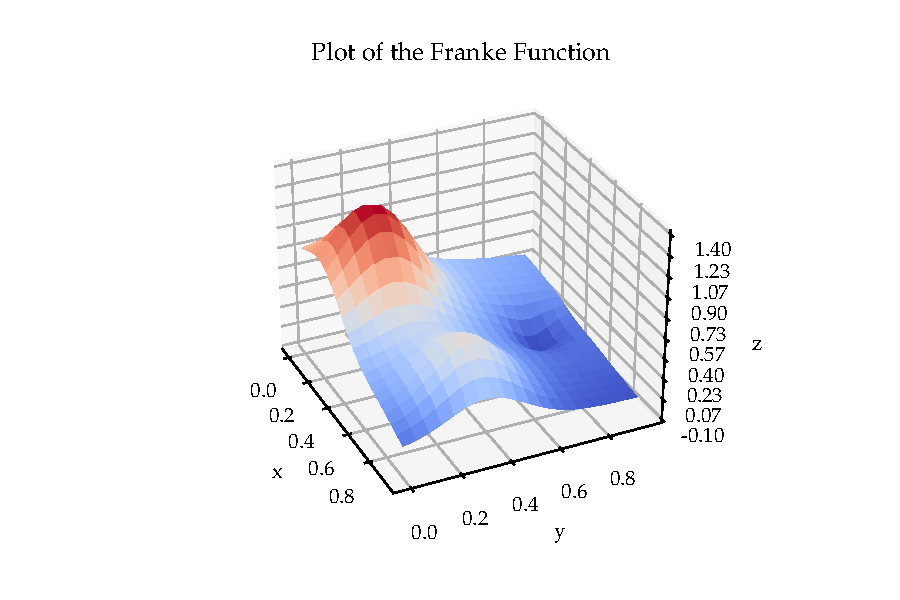
\includegraphics[scale=0.75]{figures/EX1_franke_function_nonoise_preview.pdf}
  \caption{\label{fig:1}Plot of the Franke Function}
\end{figure}

%\section*{Theory}
%The sample mean value of $\boldsymbol{y}$ is defined as;
%\begin{equation}
%    \bar{y} =  \frac{1}{n} \sum_{i=0}^{n - 1} y_i
%\end{equation}

%The sample variance of $\boldsymbol{y}$ is defined as;
%\begin{equation}
%    \mathrm{var}[\boldsymbol{x}]=\frac{1}{n}\sum_{i=0}^{n-1}(x_i- \overline{x})^2=\mathbb{E}\left[(\bm{y}-\bm{\tilde{y}})^2\right]
%\end{equation}

\section*{Exercise 1}
In Machine Learning, we are studying the problem of optimization, that is, finding the optimal parameter $\beta$ such that $C(\boldsymbol{X},\boldsymbol{\beta}) =
  {\displaystyle \min_{\boldsymbol{\beta}\in {\mathbb{R}}^{p}}}\frac{1}{n}\left\{\left(\boldsymbol{y}-\boldsymbol{X}\boldsymbol{\beta}\right)^T\left(\boldsymbol{y}-\boldsymbol{X}\boldsymbol{\beta}\right)\right\}
$ our cost function is minimized. For the following exercise, where we will study Ordinary Least Squares regression, the previously stated cost function is the one we will minimize in order to fit the Franke Function, both without (as in Figure (\ref{fig:1})) and with noise as in Figure (\ref{fig:2}).

\begin{figure}[h]
  \centering
  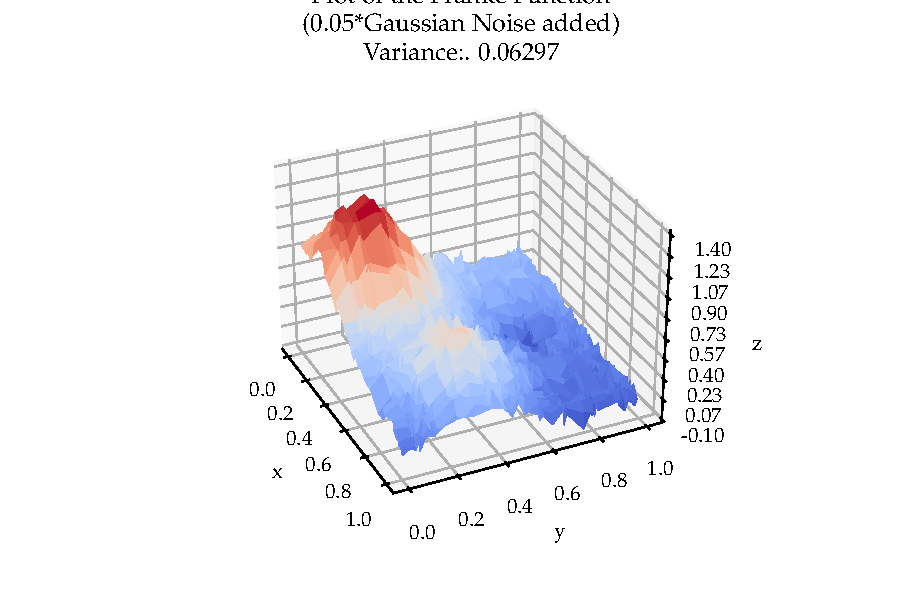
\includegraphics[scale=0.75]{figures/EX1_franke_function_noise_preview.pdf}
  \caption{\label{fig:2}Plot of the Franke Function with added stochastic noise}
\end{figure}

When constructing our OLS model, we start off by minimizing the cost function with regards to $\beta$. That is, we take the derivative of $C(\bm{X},\bm{\beta})$ and set it $0$. The following derivation shows how we end up with the optimal parameters $\bm{\hat{\beta}}$, which in turn can be used to predict new values for the function which we are fitting.

\[
  \frac{\partial{C(\boldsymbol{X},\boldsymbol{\beta})}}{\partial{\beta}} = 0
\]
\[
  \frac{\partial{C(\boldsymbol{X},\boldsymbol{\beta})}}{\partial{\beta}} = -\frac{2}{n}\bm{X}^\text{T}\left(\bm{y} - \bm{X}\bm{\beta}\right) = 0
\]
\[
  \bm{X}^\text{T}\left(\bm{y} - \bm{X}\bm{\beta}\right) = 0
\]
\[
  \bm{X}^\text{T}\bm{X}\bm{\beta} = \bm{X}^\text{T}\bm{y}
\]
\[
  \bm{\hat{\beta}} = \left(\bm{X}^\text{T}\bm{X}\right)^{-1}\bm{X}^\text{T}\bm{y}
\]
For consistency, it is noted that $\bm{\hat{\beta}} \in \mathbb{R}^p$, $\bm{y} \in \mathbb{R}^n$ and $\bm{X} \in \mathbb{R}^{n\times{p}}$.

With an expression for the predictors $\hat{\beta}$ derived, fitting a new value $\tilde{y}$ is simply $\tilde{y} = \bm{X}\bm{\hat{\beta}}$.

Our own implementation of Ordinary Least Square regression is implemented such that its use mimics that of SciKit-learn. \cite{scikit-learn} That is, we also include separate steps for initializing our model, fitting the model and predicting using the model using the just derived mathematical expression. For further inquiry about implementation, refer to the github repository linked in the \nameref{sec:A}.

\subsection*{Confidence Intervals}
Confidence intervals can be used to asses the uncertainty of a parameter. In our case, we will define confidence limits following the understanding of a Confidence Interval given in "Bootstrap Methods and their Application". That is, given a computed confidence region, any value inside the confidence region should be more likely than all values outside the confidence region. \cite{Davison1997}

Furthermore, when computing the confidence interval for the parameters $\beta$, we first compute the variance $\bm{\sigma^2}(\beta_j) = \bm{\sigma^2}\left[(\bm{X}\bm{X^\text{T}})^{-1}\right]_\text{jj}$. Where $\bm{X}\bm{X^\text{T}}$ is the Hessian matrix. Furthermore, it can be shown that the Hessian matrix can be given as the second derivative of the Cost function with respect to $\beta$. I.e.
\[
  \frac{\partial^2C}{\partial{\bm{\beta^\text{T}}}\partial{\bm{\beta}}} = \frac{2}{n}\bm{X}\bm{X^\text{T}}
\]

\subsection*{Mean Squared Error and R2 score}
Two metrics that can be used to asses the quality of a model is its Mean Square Error (MSE) and R2 score. The MSE for any estimator is defined as
\[
  \text{MSE}(\boldsymbol{y},\boldsymbol{\tilde{y}}) = \frac{1}{n}
  \sum_{i=0}^{n-1}(y_i-\tilde{y}_i)^2
\]
It will be shown later that the MSE can be broken into two components, namely the variance and the squared bias. As can be seen from the equation, the MSE would attain the value of 0 if $y_i = \tilde{y}_i$. Moreover, by rewriting the mean squared error as $\text{MSE} = \frac{1}{m}\left\lVert \bm{y} - \bm{\tilde{y}}\right\rVert_2^2$, it can be seen that the error increases as the Euclidean distance between the prediction targets increase. \cite{Goodfellow2016}

The R2 score (coefficient of determination) is another metric that can be related to how the model covers its own variance. Defined as,
\[
  \text{R}^2(\boldsymbol{y}, \tilde{\boldsymbol{y}}) = 1 - \frac{\sum_{i=0}^{n - 1} (y_i - \tilde{y}_i)^2}{\sum_{i=0}^{n - 1} (y_i - \bar{y})^2}
\] the closer the R2 score is to its maximum value 1, the more the variance of the model is explained by the model parameters. The R2 score gives a measure of model skill as a higher R2 generally indicates that the model is better at making new predictions. However, a perfect R2 score of 1 would result in the model covering it's entire variance, thus the model is overfitted and will not perform well in a general use case beyond the scope of it's initial training-data.

\todo[inline]{TODO: Possibly more one implementation} 
\todo[inline]{TODO: Add the plot showing all predicitons up to degree} 
\todo[inline]{TODO: R2 score must be plottet and briefly discussed} 

\subsection*{Scaling the data}
Our motivation for scaling the data arise in the context of fitting a design matrix of predictors with different units. To avoid having to disregard some predictors in favor of others based on their unit, not necessarily their contribution to the function fit, a scaling of the data is performed. By scaling the data using one of several scaling techniques, we ensure that all predictors lie in the same reference domain, resulting in a more accurate representation of the predictors. Furthermore, scaled data generally increases model skill. SciKit-learn includes several different Scalers, such as the StandardScaler and MinMaxScaler. \cite{scikit-learn} For this discussion, the StandardScaler will be inspected.

The idea behind scaling the data with regards to the StandardScaler method, is to subtract the mean value and then divide by the variance. By performing these two operations, we ensure that the data have a mean value equal to $0$ (i.e. are standardized/zero centered) and variance equal to $1$.
%Moreover, when scaling in this way, the intercept will be scaled by the mean value of the output. Moreover, it can be shown that zero centering leads to the new $\bm{\tilde{y}} = \bm{y} - \beta_0 = \bm{y} - \bm{\bar{y}}$, where $\bm{\bar{y}}$ is used as the sample mean of $\bm{y}$. As the columns of $\bm{X}$ also has been scaled in the same fashion, we end up the following Cost-Function
%\[
%  C(\boldsymbol{\beta}) = (\boldsymbol{\tilde{y}} - \tilde{X}\boldsymbol{\beta})^T(\boldsymbol{\tilde{y}} - \tilde{X}\boldsymbol{\beta}).  
%\]

Before scaling the dataset, an assessment of how to deal with the intercept has to be made. For reference, the intercept is defined as the first column of the design matrix, and for a polynomial fit would represent where the function intercepts with the y-axis when all other features are set to zero. Moreover, the intercept is a constant value (for our design matrices equal to 1), thus zero centering the intercept would result in a singular matrix, rendering the optimization problem unsolvable. Throughout this assignment, we are going to readd the intercept after scaling, essentially leaving the intercept untouched as to avoid any singular matrices. Moreover, for ordinary least squares regression, as there is no regularization of the predictors during the model fit, a model fitted on scaled contra unscaled data would attain the same mean squared error.

However, other regression methods such as Ridge and Lasso, which will be discussed in greater detail in further sections, have a dependance on the intercept through the hyperparamter $\lambda$ when computing their regularization term. Not including the intercept when computing the regularization term would give rise to a divergence between the mean square error for the model scaled with compared to the model scaled without the intercept. Thus, by computing the regularization term with disregard to the intercept, the first $\beta_j$ i.e. that of the intercept will be skipped in the computation. This will in most cases lead to a better mean square error for both Ridge and Lasso regression. Skipping the intercept when computing the regularization term also follows the definition of Ridge regression as in. \cite{Geron2019}

Furthermore, while on the topic of Ridge and Lasso regression, a scaling of the data should always be performed. This is due to the regularized linear models such as Ridge and Lasso being sensitive to the scale of the input features. \cite{Geron2019}

To determine whether scaling is apropriate for the current problem, that being fitting the Franke Function using oridnary least squares, an inspection of the generated data is made in light of the just discussion. For Exercise 1, the datapoints $x,y \in \left[0,1\right]$. This would indicate that the data is already scaled to a unit reference system. Moreover, as we are training a model based on the ordinary least squares, there is no dependance on scale of the input features as for regularized linear models. However, to keep the data-preprocessing consistent and to ensure that different models are comparable, we will scale the data in accordance to the StandardScaler and always remove the intercept from the design matrix. The latter to ensure that our models always have responses biased towards the origin.

\subsubsection*{Splitting the data}
As we want our model to perform well in general cases, we split the data into a training and testing set to simulate model prediction using new data. This is achieved by the aforementioned split, since the training and test data are kept entirely separated. In practice, we fit the model using the training data, then perform a test of the model using the test data. The error rate for new cases predicted by the model using the test data, can be used to understand how the model will perform on new untrained data. \cite{Geron2019} Moreover, by assessing the deviation between training error and test error, it can be seen whether the model is overfitting or not. It would be a case of overfitting if the training error is low, whereas the test error is high.

Throughout this assignment, we will split the data into a train and test set. The data could be split into an additional validation set, which is normally used for hyperparamter adjustment. However, hyperparameter adjustments are more typical for iterative optimization algorithms, typical 
gradient based methods. Therefor, we don't see any practical use for a validation set for this assignment, and we will skip out on splitting the data into an additional validation set. Generally, a validation set could be used for tuning the hyperparameter to select an optimal model, but it could also lead to suboptimal model selection caused by imprecise prediction from a too small validation set. \cite{Geron2019} Though our data consists of potentially unlimited data points, due to computational time constraints, we will resort to a relatively sparse dataset. Hence, we split into a training and test set to avoid sacrificing the training data in favor of a sufficient validation set.

Had we not omitted the validation set for hyperparameter tuning, the process of studying regularized models would have deviated somewhat from the study of the ordinary least squares regression. The process would then be that we split the data into a train-test split, as before. Moreover, the training data would have been split once more into a train and validation set, with an approximate ratio of 80 - 20 percent respectively. Furthermore, the hyperparameters are tuned with the MSE obtained from predicting using the validation set. However, as the validation set typically reports a lower error than the test set, the generalization error of the optimized model is studied using the test set. \cite{Goodfellow2016}

\subsection*{Comparing our OLS implementation to the one delivered by SciKit-learn}
With our Ordinary Least Squares model implemented as described above, we start off by benchmarking our implementation to the LeastSquares method found in SciKit-learn. \cite{scikit-learn} We start off by setting up a uniform 2-dimensional grid and initialize a Franke Function with some added stochastic noise.

\begin{lstlisting}
  np.random.seed(4155)
  n = 100 # The number of points in direction for the Franke Function
  x = np.sort(np.random.uniform(0, 1, n))
  y = np.sort(np.random.uniform(0, 1, n))
  x, y = np.meshgrid(x,y)
  z = FrankeFunction(x, y) + noise_factor(n,factor=0.05)
\end{lstlisting}

For this initial run, we are interested in studying the least squares fit of the Franke Function up to the fifth order.

\begin{figure}[h]
  \centering
  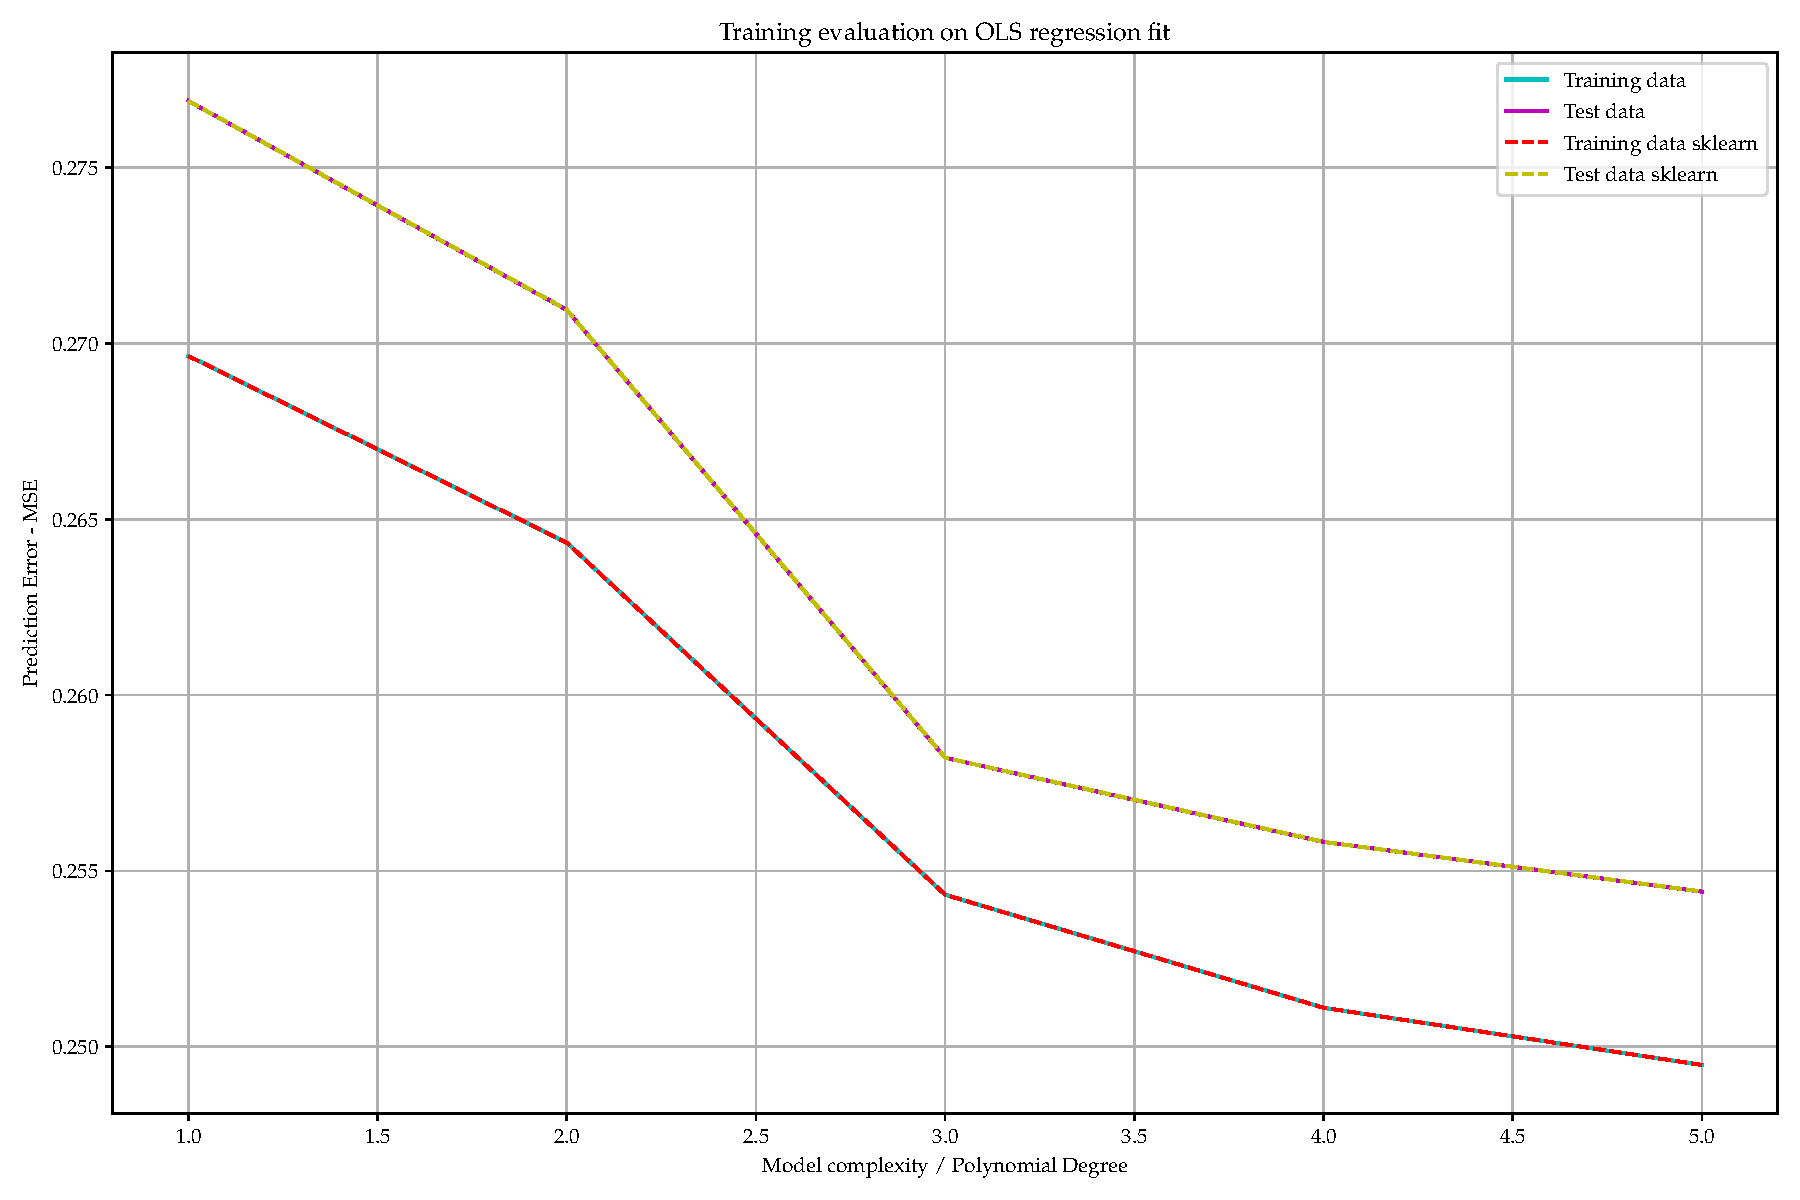
\includegraphics[scale=0.5]{figures/EX1_franke_function_OLS_evaluate_fit_1.pdf}
  \caption{\label{fig:OLS_franke_1} Benchmark run of the Franke Function fit with added Gaussian noise (factor of 0.05) with degree up to the fifth order of our OLS implementation compared to the similar LinearRegression() from SciKit-learn}
\end{figure}

By inspecting Figure (\ref{fig:OLS_franke_1}), we can see that there are no visual differences between our implementation of OLS compared to the SciKit-learn implementation. Moreover, there is a reduction in MSE as model complexity increases. Thus it is clear that a higher order fit of the model results in a lower prediction error when predicting new values using the train and test data. Moreover, as higher order polynomials are not currently studied for this initial run, at which degree the model would start to overfit is not currently known.

\begin{figure}
  \centering
  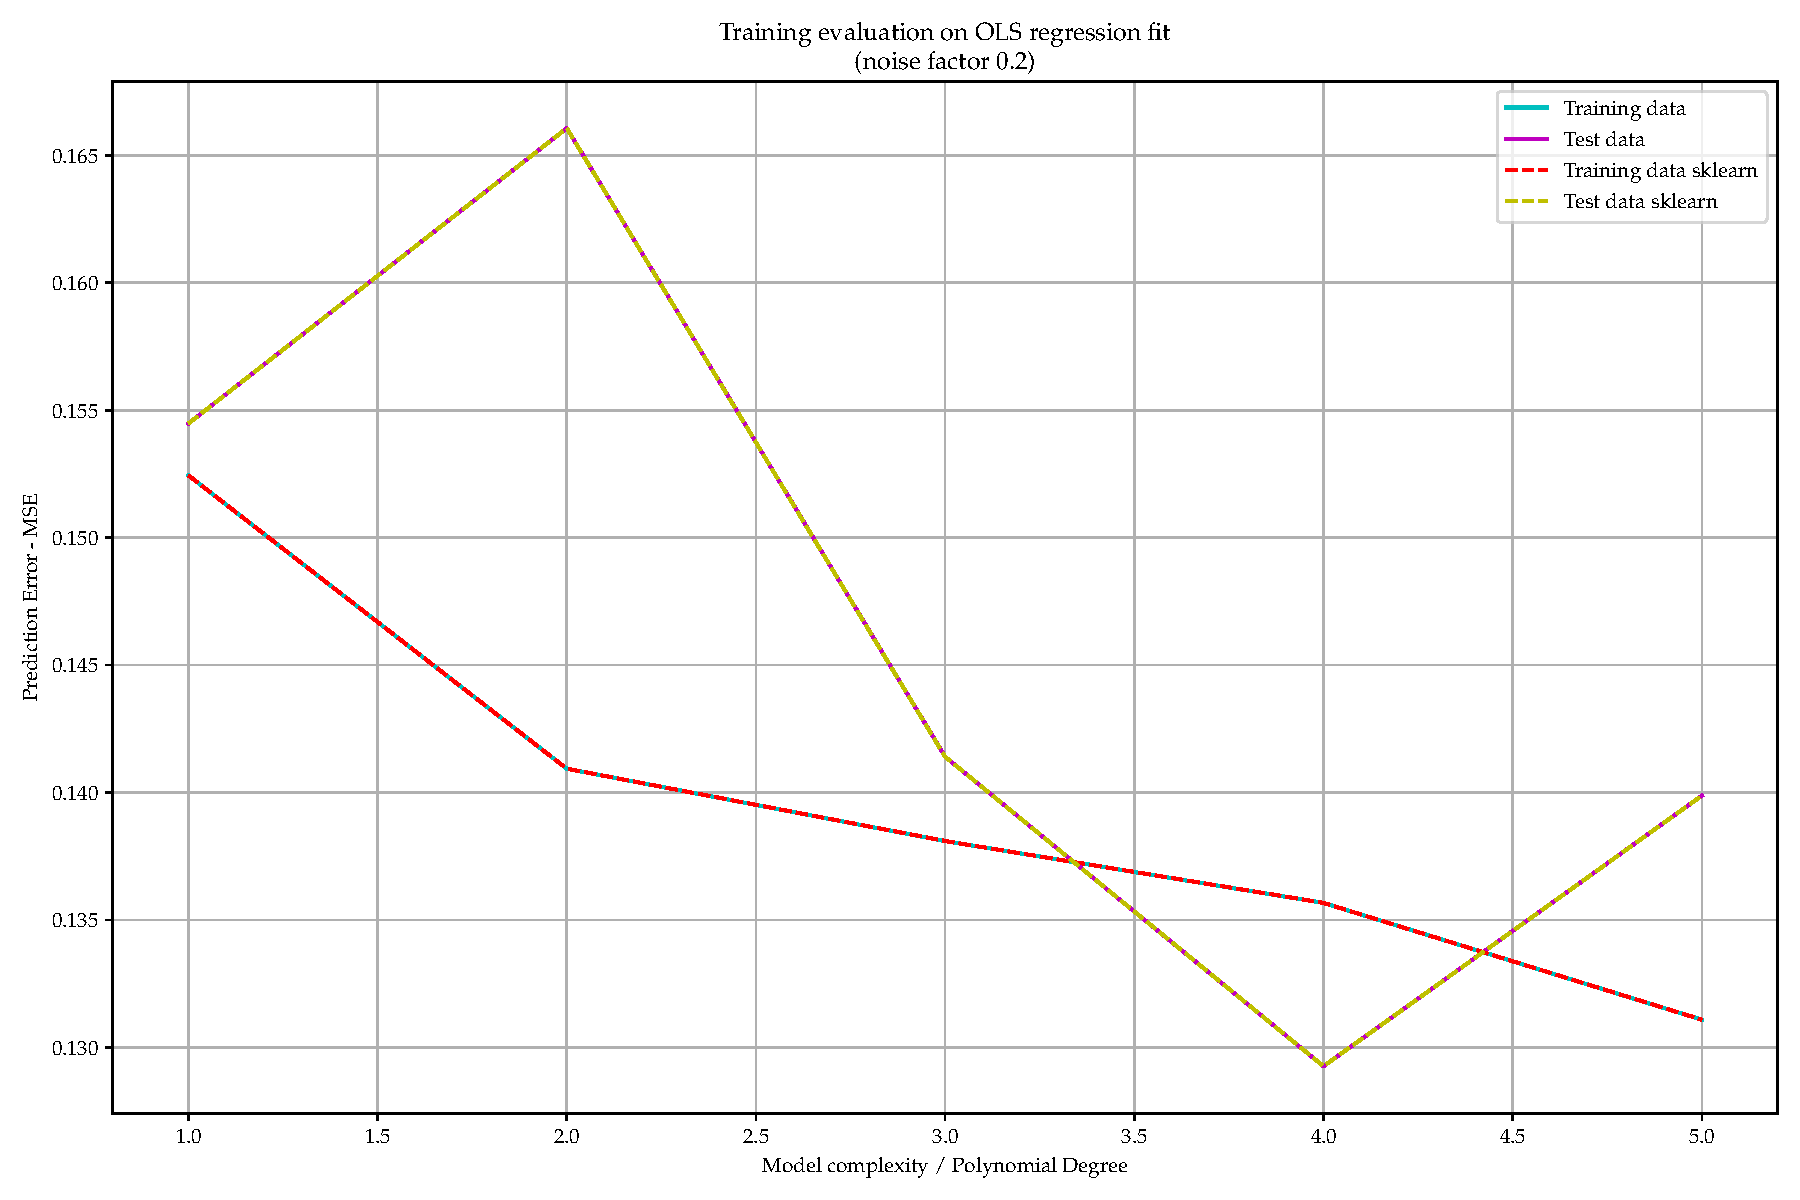
\includegraphics[scale=0.5]{figures/EX1_franke_function_OLS_evaluate_fit_dn.pdf}
  \caption{\label{fig:OLS_franke_2} Benchmark run with four times the amount of added Gaussian noise (factor of 0.2) of our OLS implementation to the similar LinearRegression() from SciKit-learn}
\end{figure}

Comparing Figure (\ref{fig:OLS_franke_1}) and (\ref{fig:OLS_franke_2}), where the first figure features a quarter the amount of added noise compared to the second figure, there are two things of note. Firstly, Figure (\ref{fig:OLS_franke_1}) attains an overall lower MSE, even as the order of the fitted function increases. Secondly, the two figures (\ref{fig:OLS_franke_2}) and (\ref{fig:OLS_franke_1}), seem to somewhat attain the same shape for both the prediction and test error. As such, we make a preliminary conclusion that fitting functions with a higher amount of added Gaussian noise is more difficult than for smooth "predictable" functions.

The Confidence Interval for the predictors $\beta_j$ is constructed for both model fits with up to fifth order polynomials. As the predictors are based not only of the x and y parameters in isolation, but also their interaction terms, a fifth order fitted model includes 21 different predictors. The result of computing the Confidence Interval for the 21 different predictors can be seen in Figure (\ref{fig:OLS_beta_1}) and (\ref{fig:OLS_beta_2}). From Figure \ref{fig:OLS_beta_1}, it can be seen that the lowermost and higher order terms have the smallest confidence intervals. Thus some of the predictors related to x and y of the third and fourth order pose the highest uncertainty. Furthermore, comparing Figure (\ref{fig:OLS_beta_1}) to (\ref{fig:OLS_beta_2}) shows that as the added noise is increased in size, the uncertainty of the predictors is increased as seen in the slightly larger confidence intervals. The predictor values also attain slightly altered values, though their general position in relation to each other seems to be preserved.

\begin{figure}
  \centering
  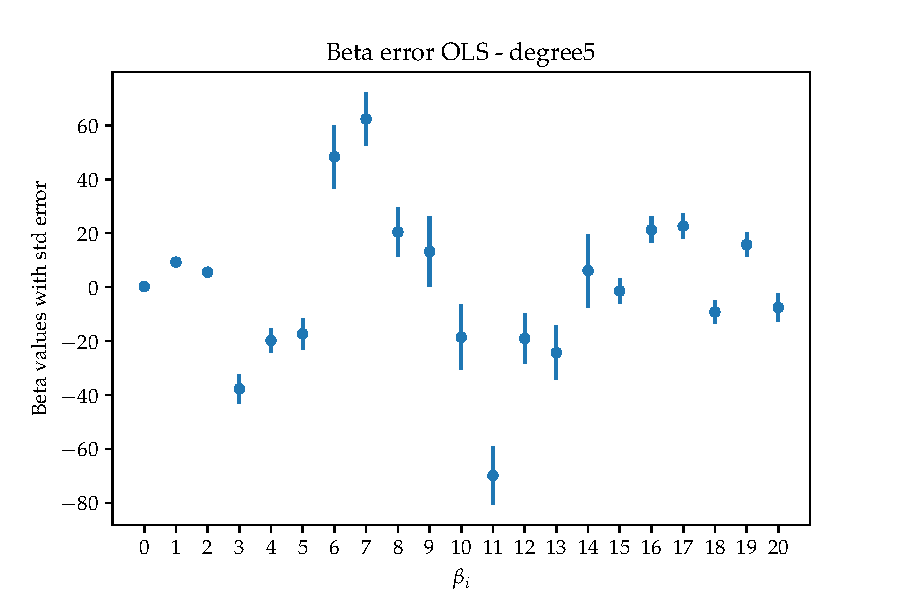
\includegraphics[scale=.85]{figures/EX1_OLS_beta_error_degree5.pdf}
  \caption{\label{fig:OLS_beta_1} 95\% Confidence intervals for the predictors of an OLS model with polynomials up to the fifth order and added Gaussian noise multiplied with a factor of 0.05.}
\end{figure}

\begin{figure}
  \centering
  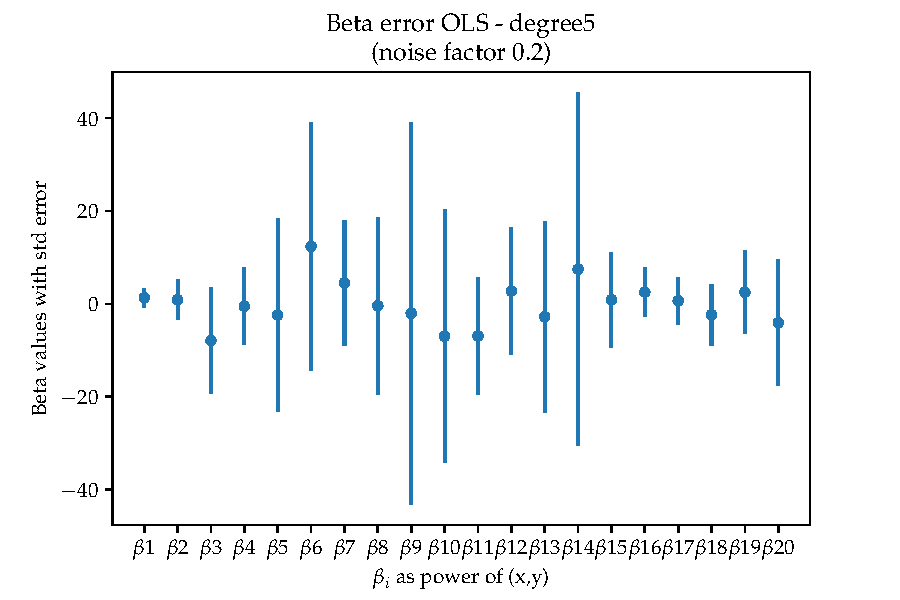
\includegraphics[scale=.85]{figures/EX1_OLS_beta_error_degree5_mn.pdf}
  \caption{\label{fig:OLS_beta_2} 95\% Confidence intervals for the predictors of an OLS model with polynomials up to the fifth order and added Gaussian noise multiplied with a factor of 0.1.}
\end{figure}

Following the comparison of Figure (\ref{fig:OLS_franke_1}) and (\ref{fig:OLS_franke_2}), comparing the two confidence intervals reveals that as the added Gaussian noise is increased in size, the confidence intervals for the predictors increase as well. This can be seen especially for the predictors with some variability for the $0.05$ noise factor case. Thus, as we increase the Gaussian noise added to the Franke Function, our predictors become less uncertain, which in turn could result in less precise model predictions.

For the rest of this assignment up to and including Exercise 5, we will add noise with a factor of $0.2$ to all our data, unless otherwise stated.

%\begin{figure}
%  \centering
%  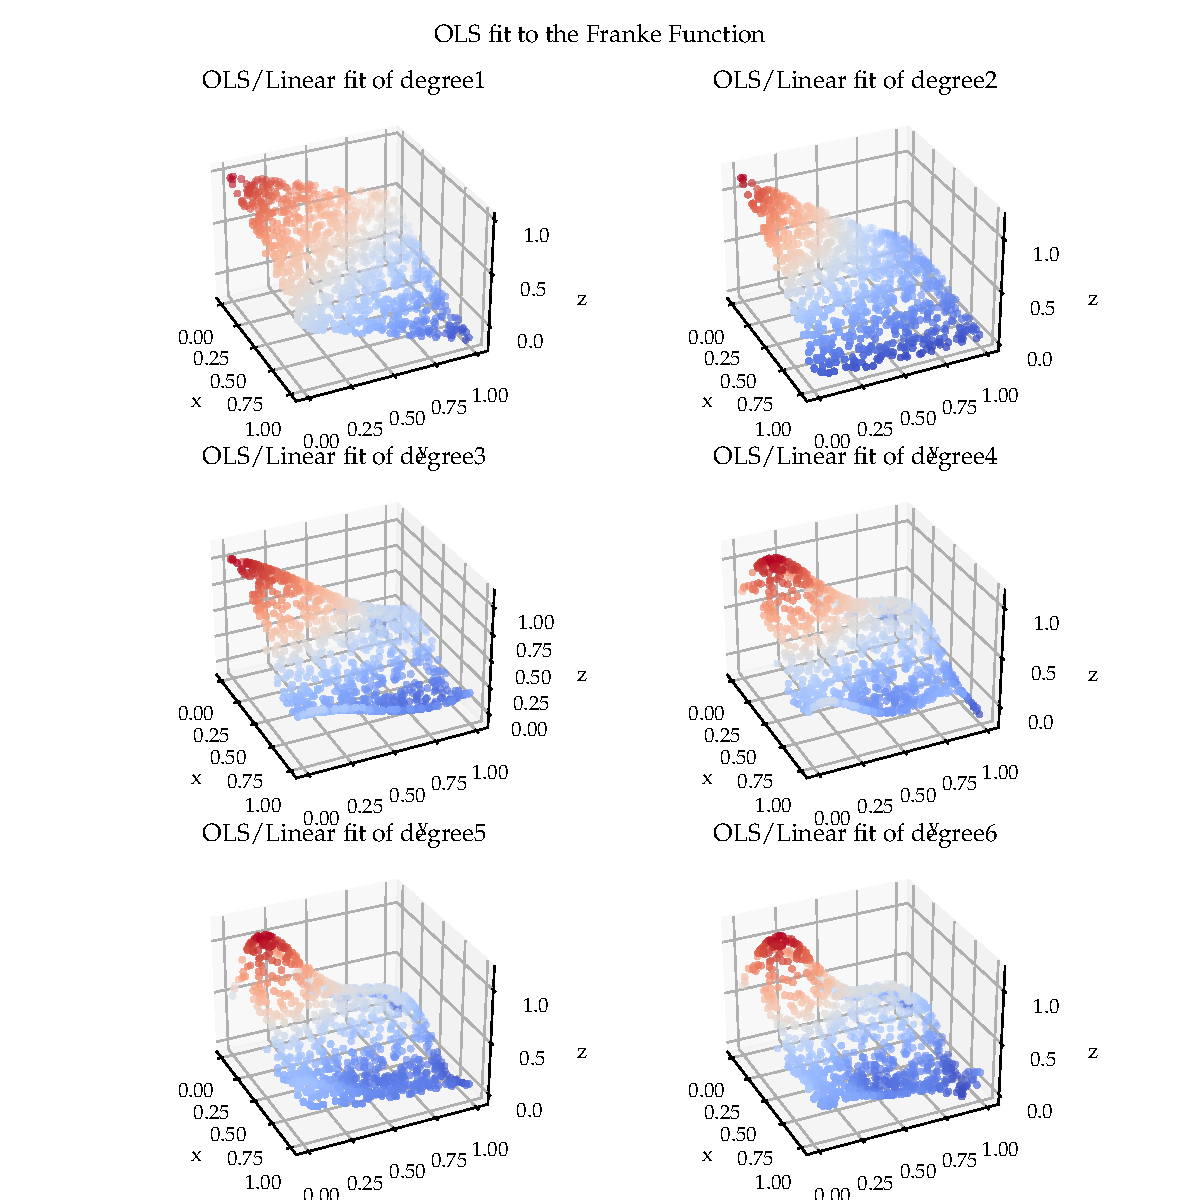
\includegraphics[scale=0.85]{figures/franke_function_OLS_fit.pdf}
%  \caption{?}
%  \label{fig:3}
%\end{figure}

%\begin{figure}
%  \centering
%  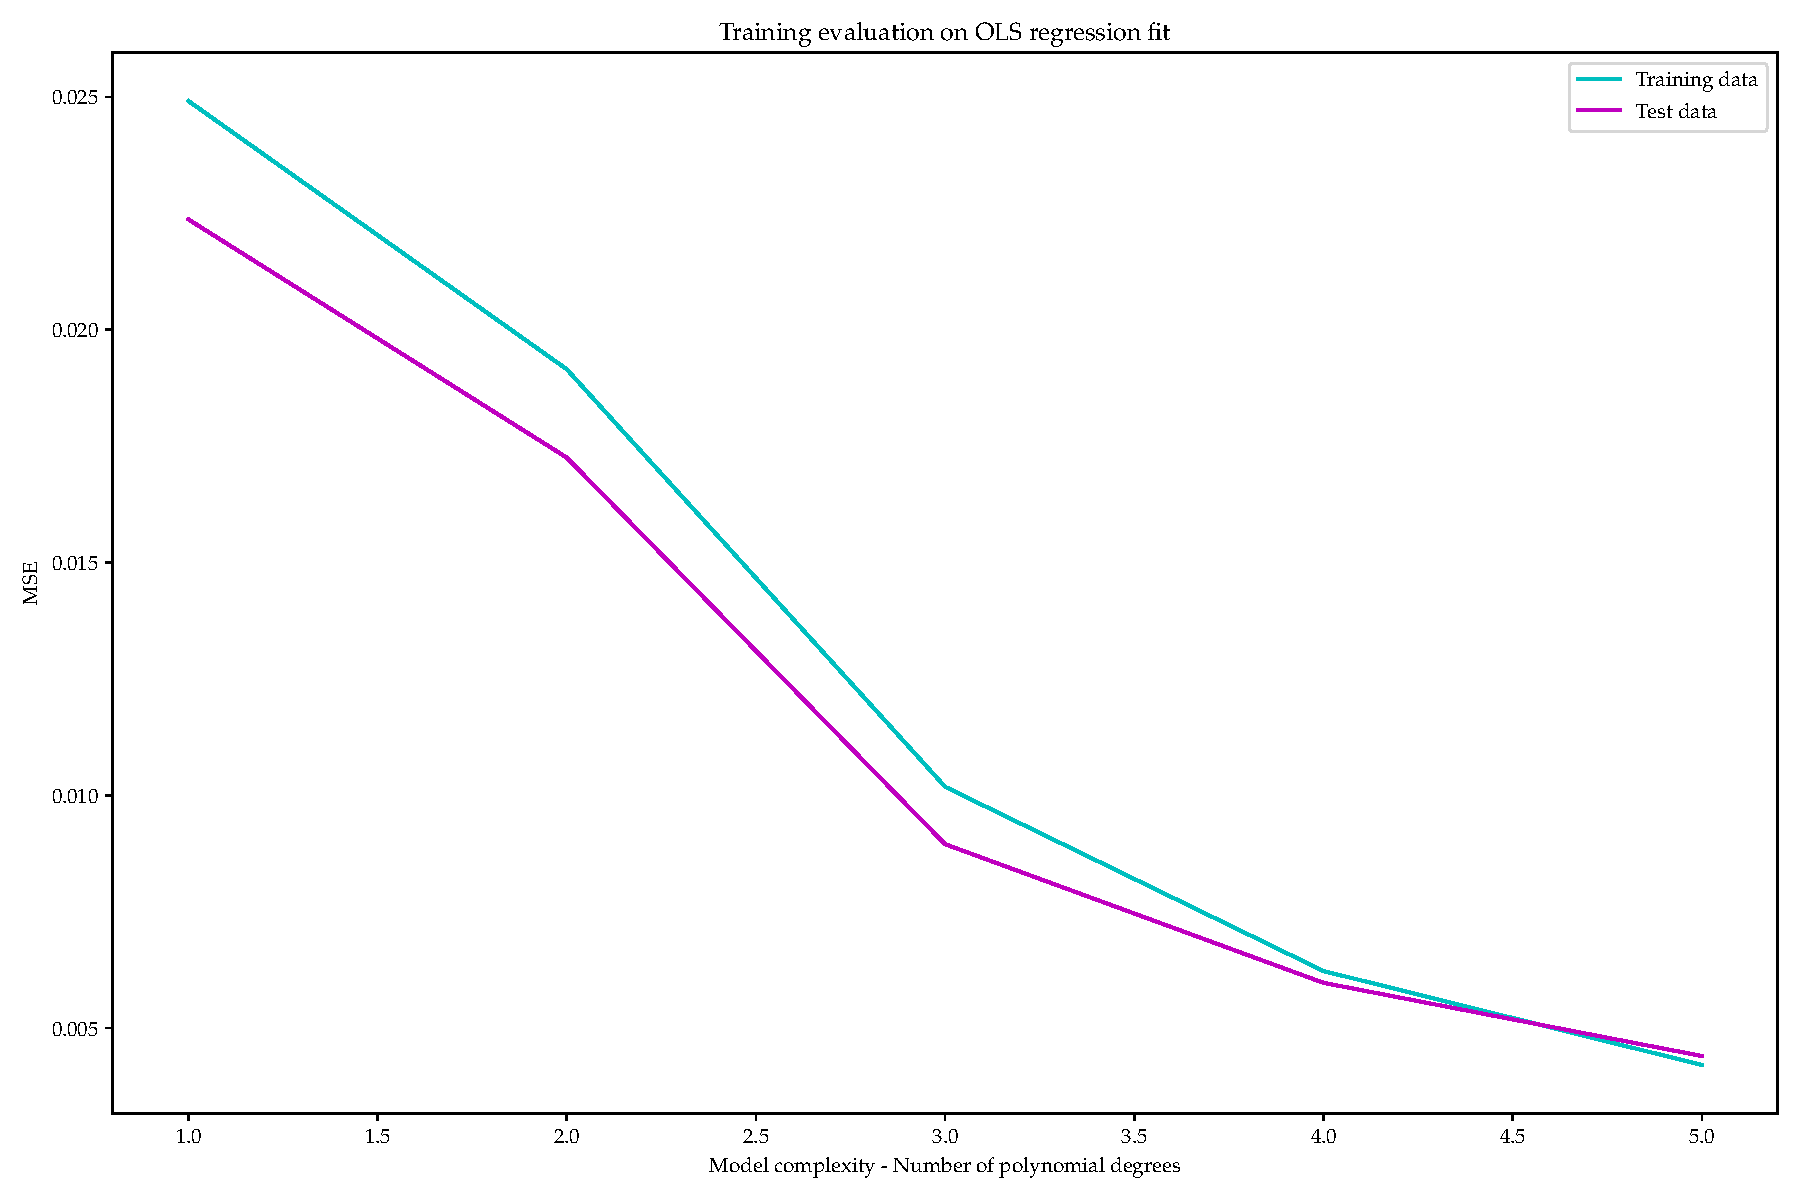
\includegraphics[scale=0.45]{figures/franke_function_OLS_evaluate_fit.pdf}
%  \caption{?}
%  \label{fig:4}
%\end{figure}

%\begin{figure}
%  \centering
%  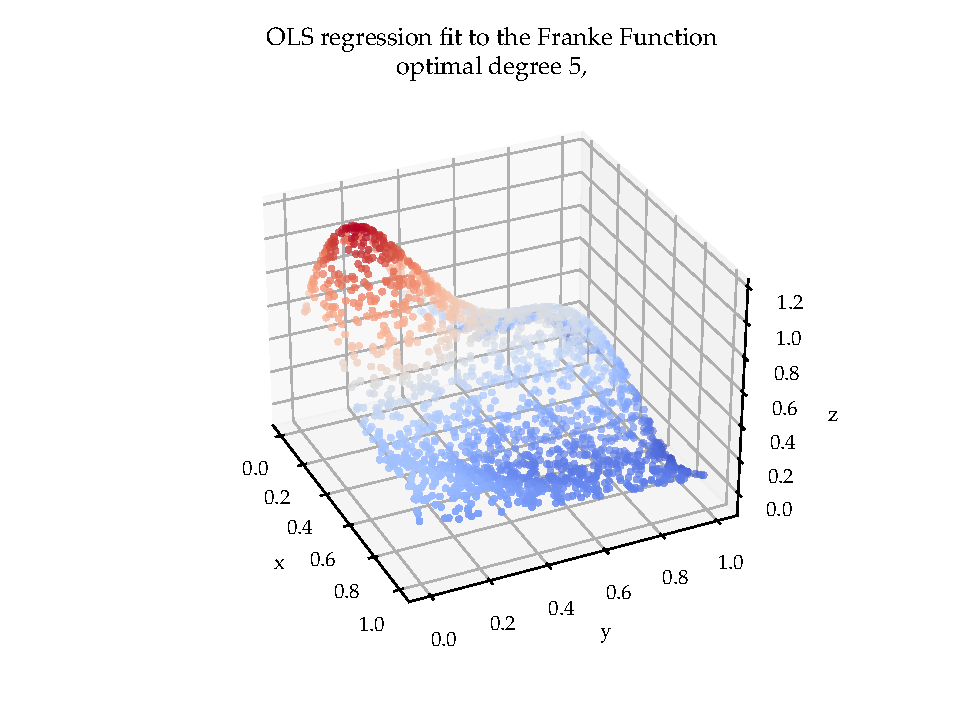
\includegraphics[scale=0.85]{figures/franke_function_OLS_best_fit.pdf}
%  \caption{?}
%  \label{fig:5}
%\end{figure}


\section*{\label{ex:2}Exercise 2}


\subsection*{The bias-variance trade-off analysis}

Moving on to the bias-variance trade-off analysis, we start off by showing that
\todo[inline]{TODO: add new figure9 with different test size. Comment on results and compare}
\[
  C(\bm{X},\bm{\beta}) =\frac{1}{n}\sum_{i=0}^{n-1}(y_i-\tilde{y}_i)^2=\mathbb{E}\left[(\bm{y}-\bm{\tilde{y}})^2\right]
\]

Can be rewritten as

\[
  \mathbb{E}\left[(\bm{y}-\bm{\tilde{y}})^2\right]=\frac{1}{n}\sum_i(f_i-\mathbb{E}\left[\bm{\tilde{y}}\right])^2+\frac{1}{n}\sum_i(\tilde{y}_i-\mathbb{E}\left[\bm{\tilde{y}}\right])^2+\sigma^2.
\]

where the terms are respectively $(\text{bias})^2$, variance and noise. For simplicity, assume that we have a dataset where the data is generated from a noisy model

\[\bm{y} = f(\bm{x}) + \bm{\epsilon}\]

Furthermore, we will assume that the residuals $\epsilon$ are independant and normally distributed $\epsilon \sim \mathcal{N}(0, \sigma^2)$. Finally, $\bm{\tilde{y}} = \bm{X}\bm{\beta}$ is our approximation to the functions $f$. Start off by adding and subtracting $\mathbb{E}\left[\bm{\tilde{y}}\right]$ inside the expectation value.

\[
  \mathbb{E}\left[(\bm{y}-\bm{\tilde{y}})^2\right]
  = \mathbb{E}\left[(\bm{y}-\bm{\tilde{y}} + \mathbb{E}\left[\bm{\tilde{y}}\right] - \mathbb{E}\left[\bm{\tilde{y}}\right])^2\right]
\]
\[
  = \mathbb{E}\left[((\bm{y} - \mathbb{E}\left[\bm{\tilde{y}}\right]) - (\bm{\tilde{y}} - \mathbb{E}\left[\bm{\tilde{y}}\right]))^2\right]
\]
By using the fact that $\bm{y} = f(\bm{x}) + \bm{\epsilon}$
we can rewrite this as
\[
  = \mathbb{E}\left[((f(\bm{x}) - \mathbb{E}\left[\bm{\tilde{y}}\right]) - (\bm{\tilde{y}} - \mathbb{E}\left[\bm{\tilde{y}}\right]) + \epsilon)^2\right]
\]
Computing the square inside the expectation value gives us
\[
  = \mathbb{E}\left[(f(\bm{x}) - \mathbb{E}\left[\bm{\tilde{y}}\right])^2 + (\bm{\tilde{y}} - \mathbb{E}\left[\bm{\tilde{y}}\right])^2 + \epsilon^2 \right]\]
\[+ 2\left(\mathbb{E}\left[\epsilon(f(\bm{x}) - \mathbb{E}\left[\bm{\tilde{y}}\right])\right]- \mathbb{E}\left[\epsilon(\bm{\tilde{y}} - \mathbb{E}\left[\bm{\tilde{y}}\right])\right] - \mathbb{E}\left[(f(\bm{x}) - \mathbb{E}\left[\bm{\tilde{y}}\right])(\bm{\tilde{y}} - \mathbb{E}\left[\bm{\tilde{y}}\right])\right]\right)
\]
Moreover, as $\epsilon$ are independant variables, the expectation value involving them as a product can be written as a product of expectation values. Knowing that $\mathbb{E}\left[\epsilon\right] = 0$, the third and second to last term is equal to zero. Also, knowing that $\mathbb{E}\left[\bm{\tilde{y}}\right] = \bm{\tilde{y}}$, the last t

\begin{equation}\label{eq:varbi}
  = \mathbb{E}\left[(f(\bm{x}) - \mathbb{E}\left[\bm{\tilde{y}}\right])^2\right] + \mathbb{E}\left[(\bm{\tilde{y}} - \mathbb{E}\left[\bm{\tilde{y}}\right])^2\right] + \mathbb{E}\left[\epsilon^2 \right]
\end{equation}
The first term in (\ref{eq:varbi}) can be discretized as
\[
  \mathbb{E}\left[(f(\bm{x}) - \mathbb{E}\left[\bm{\tilde{y}}\right])^2\right] = \frac{1}{n}\sum_i(f_i - \mathbb{E}\left[\bm{\tilde{y}}\right])^2
\]
Which is the bias squared as we were to show.

The second term in (\ref{eq:varbi}) is also discretized, yielding
\[
  \mathbb{E}\left[(\bm{\tilde{y}} - \mathbb{E}\left[\bm{\tilde{y}}\right])^2\right] = \frac{1}{n}\sum_i(\bm{\tilde{y}} - \mathbb{E}\left[\bm{\tilde{y}}\right])^2
\]
Which takes form of the variance, as was set out to show.

Finally, it can be shown that $\text{var}(\bm{y}) = \text{var}(f + \epsilon) = \mathbb{E}\left[(f + \epsilon)^2\right] - (\mathbb{E}\left[(f + \epsilon)\right])^2$ = $\mathbb{E}\left[\epsilon^2\right]$ As such, we can use that \[
  \text{var}(y) = \sigma^2 = \mathbb{E}\left[\epsilon^2\right]
\]
to see that the final term in (\ref{eq:varbi}) is equal to the noise. Thus we have shown that
\[
  \mathbb{E}\left[(\bm{y}-\bm{\tilde{y}})^2\right] = \mathbb{E}\left[(f(\bm{x}) - \mathbb{E}\left[\bm{\tilde{y}}\right])^2\right] + \mathbb{E}\left[(\bm{\tilde{y}} - \mathbb{E}\left[\bm{\tilde{y}}\right])^2\right] + \mathbb{E}\left[\epsilon^2 \right]
\]
\[
  =\frac{1}{n}\sum_i(f_i-\mathbb{E}\left[\bm{\tilde{y}}\right])^2+\frac{1}{n}\sum_i(\tilde{y}_i-\mathbb{E}\left[\bm{\tilde{y}}\right])^2+\sigma^2.
\]

The final expression consists of three terms. The first term is a sum of the squared bias, the second term is the variance and the final term is a constant noise term. The sum of squared bias and variance make up the mean square error of our model. \cite{Hastie2009}

The bias component of the mean square error measures the difference from the true mean to the desired regression model. As function of model complexity, the bias will decrease as complexity increases. The second term, the variance, gives a measurement of the variation of the model values around their average value. The variance will increase with model complexity. The constant noise term $\sigma^2$ is an irreducible error which can only be reduced by cleaning up the data beforehand. \cite{Geron2019}. As the irreducible error is out of our control, it does not contribute when analyzing the bias-variance tradeoff.

The bias-variance tradeoff can be used as a method for model selection. As has been alluded to in the previous paragraph, the variance is inverse proportional to the bias. As such, there is a trade-off between bias and variance. As the bias-variance is directly related to the mean square error for both the training data but also test and production data used for making new predictions. When selecting a model we wish to balance and minimize both quantities, as that leads to the model with the best predicitve capabilities. \cite{Bishop2016}

Furthermore, the problem of overfitting can also be discussed in light of the bias variance tradeoff. Overfitting is proportional to the model variance, as such a high variance leads to an overfitted model. An overfitted model is one that has learned the noise of the training data, resulting in a perfect fit for the training data but a high mean square error when predicting using new data. Hence, a higher bias can be considered more useful to circumvent overfitting.

Lastly, it should be noted that the bias-variance tradeoff measuremnet is performed for a single dataset of limited size. As such, if there were more datapoints to train the model with, the model would attain a better overall fit. Moreover, a greater amount of training data would reduce the level of overfitting for a given model complexity. \cite{Bishop2016} Though there are some limitations to the measurement, the bias-variance tradeoff can be used to estimate where the trained model is general enough to both avoid under -and overfitting (i.e. too high bias or too high variance).

%\begin{figure}
%  \centering
%  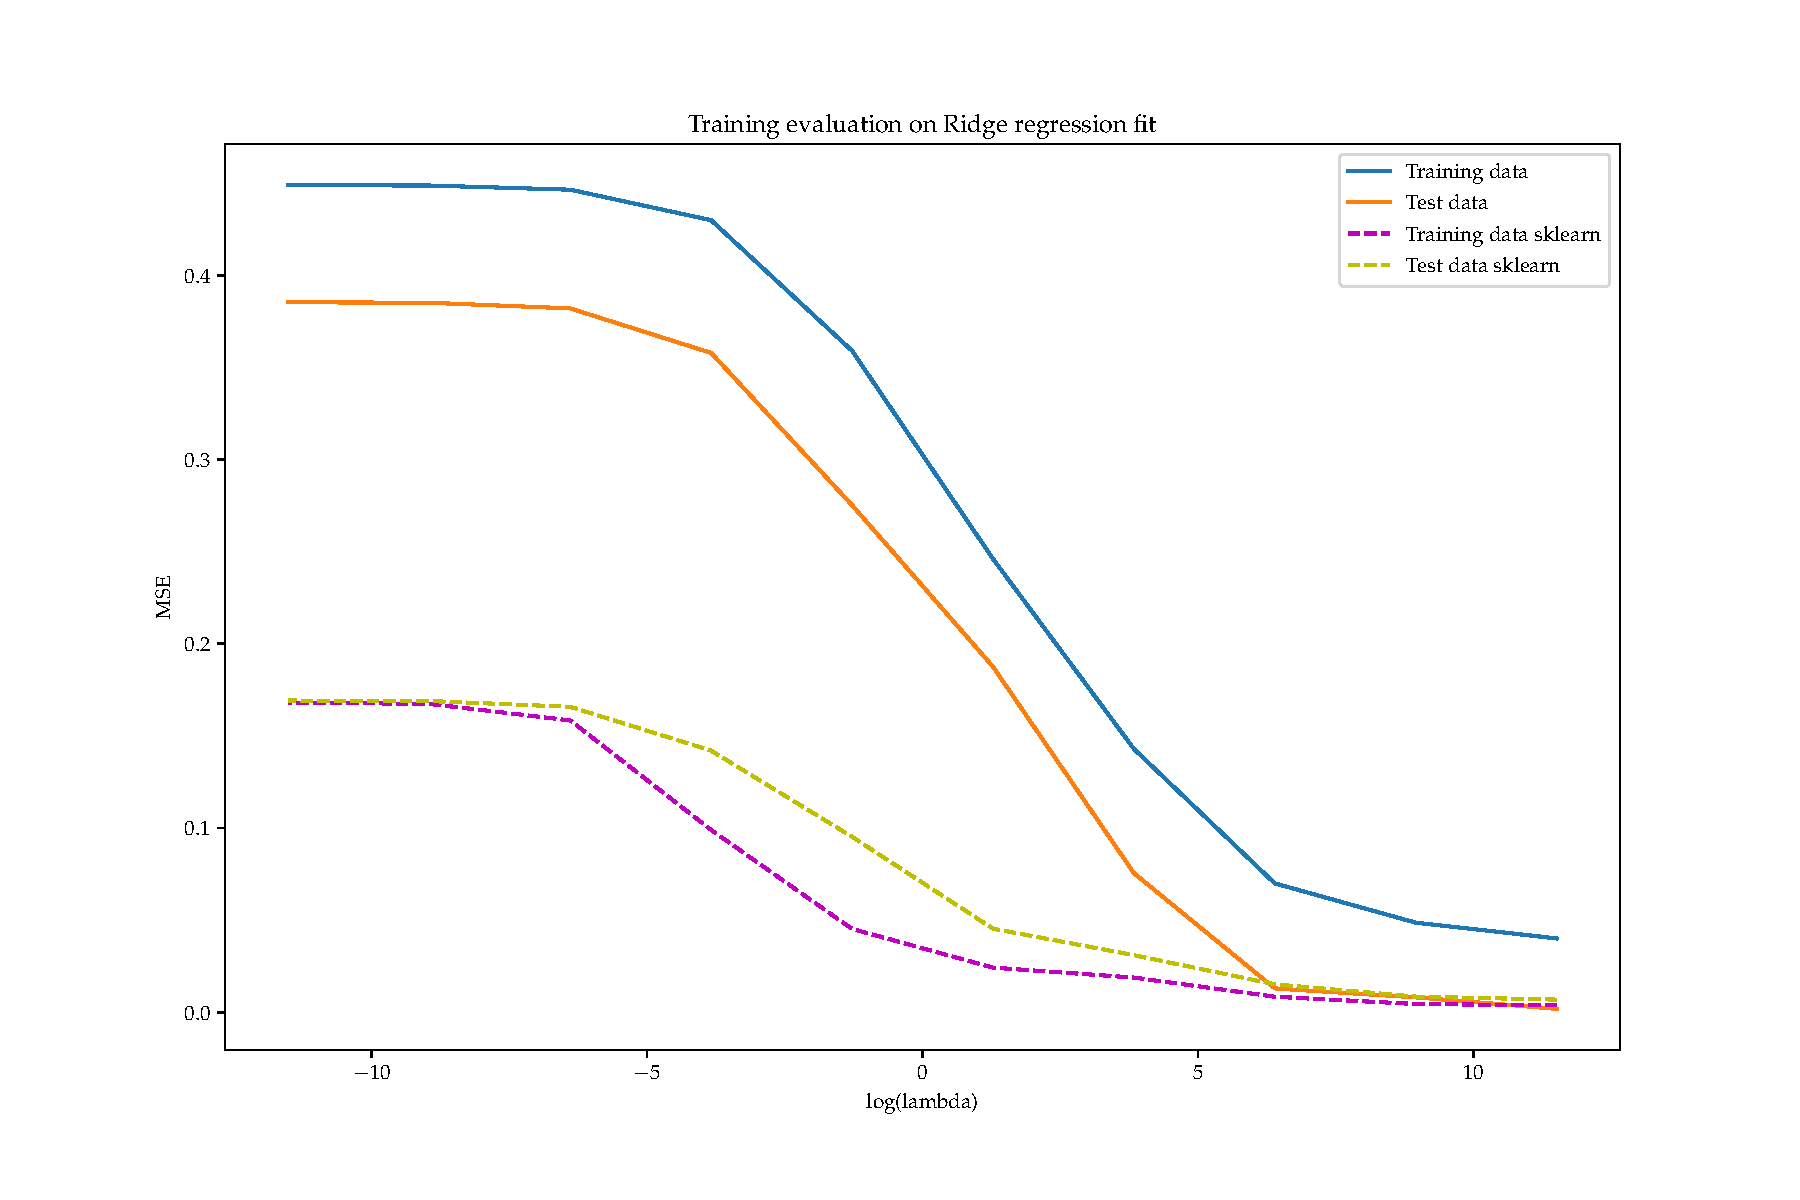
\includegraphics[scale=0.45]{figures/franke_function_Ridge_evaluate_fit.pdf}
%  \caption{The best fit using Ridge}
%  \label{fig: Ridge_best_fit}
%\end{figure}

%\begin{figure}
%  \centering
%  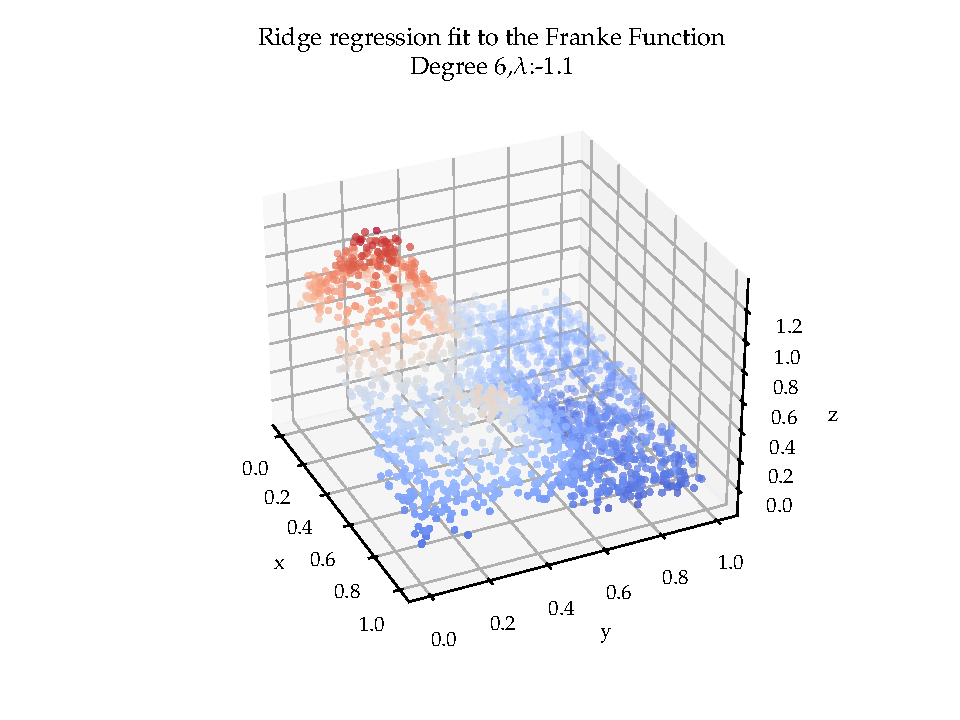
\includegraphics[scale=0.85]{figures/franke_function_Ridge_best_fit.pdf}
%  \caption{The best fit using Ridge}
%  \label{fig: Ridge_best_fit_2}
%\end{figure}

%\begin{center}
%  \csvautobooktabular{data/report_data/redge_reg_lambda_-1.1.csv}
%  \label{data: Ridge_best_fit}
%\end{center}

\begin{figure}
  \centering
  \begin{subfigure}{0.49\textwidth}
      \centering
      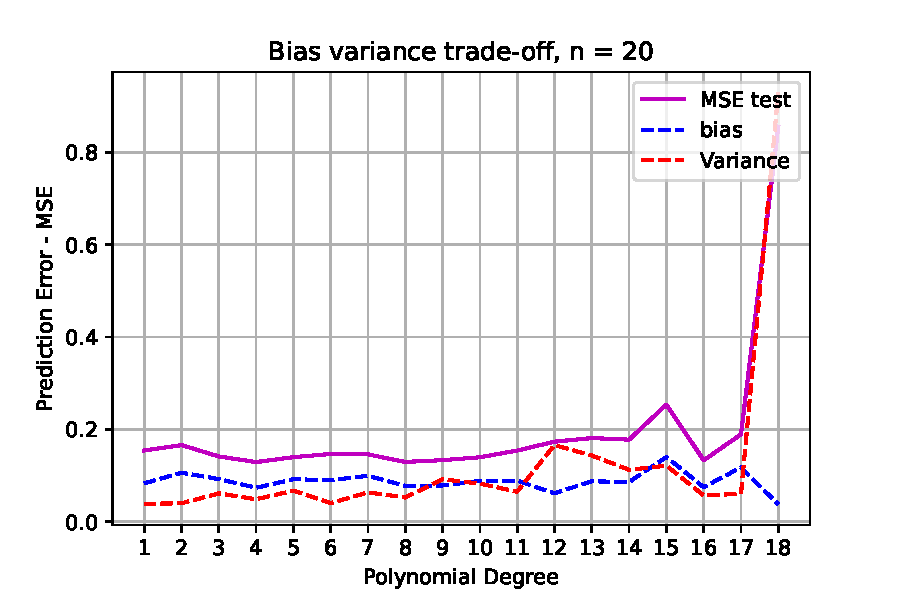
\includegraphics[width=\textwidth]{figures/EX2_model_complexity_bias_var_function_n_20.pdf}
      \caption{400 datapoints}
      \label{fig:bias_var_n_20}
  \end{subfigure}
  \hfill
  \begin{subfigure}{0.49\textwidth}
      \centering
      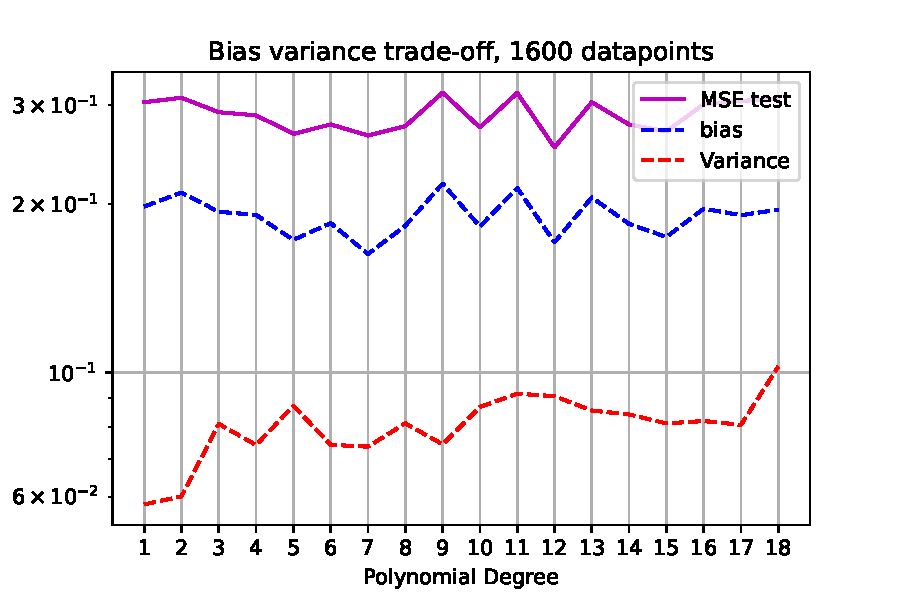
\includegraphics[width=\textwidth]{figures/EX2_model_complexity_bias_var_function_n_40.pdf}
      \caption{1600 datapoints}
      \label{fig:bias_var_n_30}
  \end{subfigure}

     \caption{Bias variance trade-off as function of number of datapoints and model complexity}
     \label{fig:bias_var}
\end{figure}


Figure 7(a) visualizes a polynomial degree where this point lies within the given model.  With a dataset consisting of 400 data points, one can see a rapid increase in variance at degree 11. Here the model is starting to produce results that deviate from the expected estimator values. At degree 17, there is a drastic increase in the variance, while the bias is moving towards zero. This is clear evidence of the model being overfitted to the training data. 

On the other hand, increasing the dataset to contain 1600 data points produces completely different results. The percentage of data used in training is kept constant between these two examples, resulting in the increase from 320 data points to 1280. This gives the model a significantly better foundation for generalizing on the data, hence resulting in a much lower MSE at the degrees in the higher range of the interval in question. At this number of data points, there is still no clear evidence of overfitting.  

\subsection*{Some words on bootstrapping}
As described in the preceding task, we split our data into several subsets used for different purposes. The overall objective is to train a model on a given subset and then measure how well it performs on a new unseen data set. However, a dilemma that may emerge from this approach is that our data only represents a sample from an unknown distribution. We run the risk of measuring a predicted error that deviates from the actual probability by iterating through our data points only once.

Therefore, we impose resampling methods on our data to produce a more realistic estimate of the error.This will help us in the the process of assesing the model. The following algorithm will demonstrate how the bootstrap is performed to achieve this:

We have some data, which consists of training data:

$$X = [x_1,x_2,...,x_n]$$
and their respective target labels:
$$\bm{y} = [y_1,y_2,...,y_n]$$


(I) A new sample is then drawn. This dataset will have the same dimension as D, but as it is drawn with replacements, they will differ from eachother as the latter has a probability of drawing the same sample mulitple times:

$$X^* = x_{1}^{*}, x_{2}^{*}, ... ,x_{n}^{*}$$
$$\bm{y}^*= y_{1}^{*}, y_{2}^{*}, ... ,y_{n}^{*}$$

(II)This sample is then used to create new set of predictors:
\[
  \bm{\hat{\beta}}^* = \left(\bm{X}^\text{*T}\bm{X}^*\right)^{-1}\bm{X}^\text{*T}\bm{y}^*
\]

(III)which in turn is used to predict new values on our test data. It is of great importance to emphasize that that $X_{test}$ is completly seperated from the rest of data, and only used to predict the new values for each sample.


$$\tilde{y}^* = \bm{X}_{test}\bm{\hat{\beta}^*}$$.

(IV)We then compute the error in our predictions:
\[
  \text{MSE}(\boldsymbol{y},\boldsymbol{\tilde{y}^*}) = \frac{1}{n}
  \sum_{i=0}^{n-1}(y_i-\tilde{y}^{*}_i)^2
\]

Step I-IV is then repeated $B$ times, while keeping track of each sample MSE. After the completion of B bootstraps, an average of all MSE´s is calculated. Ideally, B is less than the number of datapoints. This is implemented in our algorith by simply setting B to some fraction of the size of the data set. 


\begin{figure}
  \centering
  \begin{subfigure}{0.49\textwidth}
      \centering
      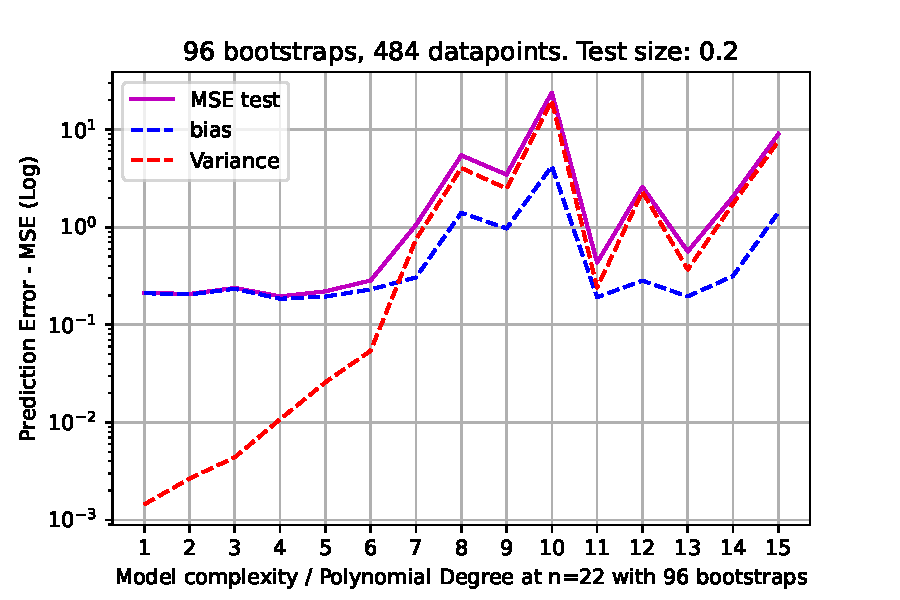
\includegraphics[width=\textwidth]{figures/EX2_model_complexity_using_bootstrap_function_n_22_testsize_0.2.pdf}
      \caption{400 datapoints, 200 bootstraps}
      \label{fig:bootstrap_bias_var_n_20}
  \end{subfigure}
  \hfill
  \begin{subfigure}{0.49\textwidth}
      \centering
      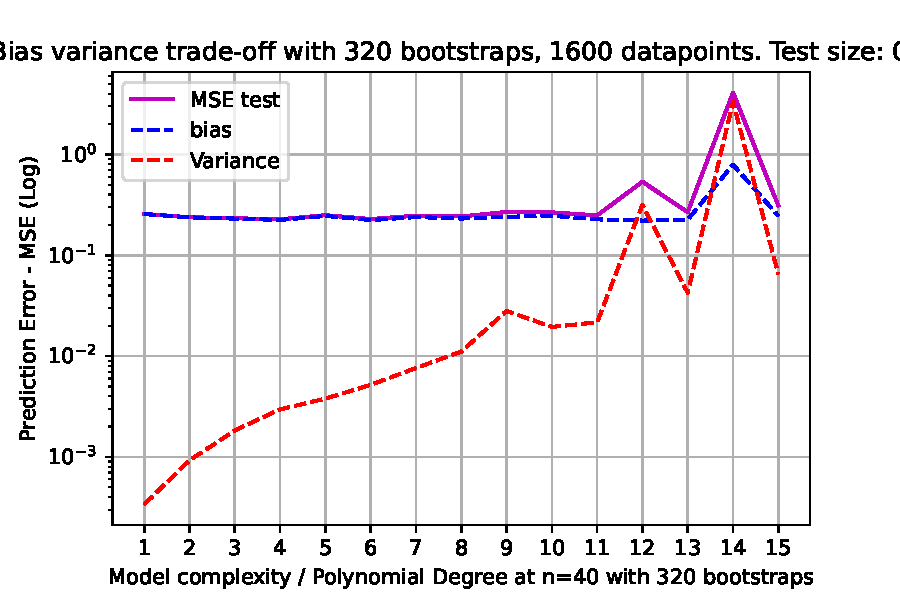
\includegraphics[width=\textwidth]{figures/EX2_model_complexity_using_bootstrap_function_n_40_testsize_0.2.pdf}
      \caption{1600 datapoints, 800 bootstraps}
      \label{fig:bootstrap_bias_var_n_30}
  \end{subfigure}

     \caption{Bias variance trade-off with bootstrap}
     \label{fig:bootstrap_bias_var}
\end{figure}



\begin{figure}
  \centering
  \begin{subfigure}{0.49\textwidth}
      \centering
      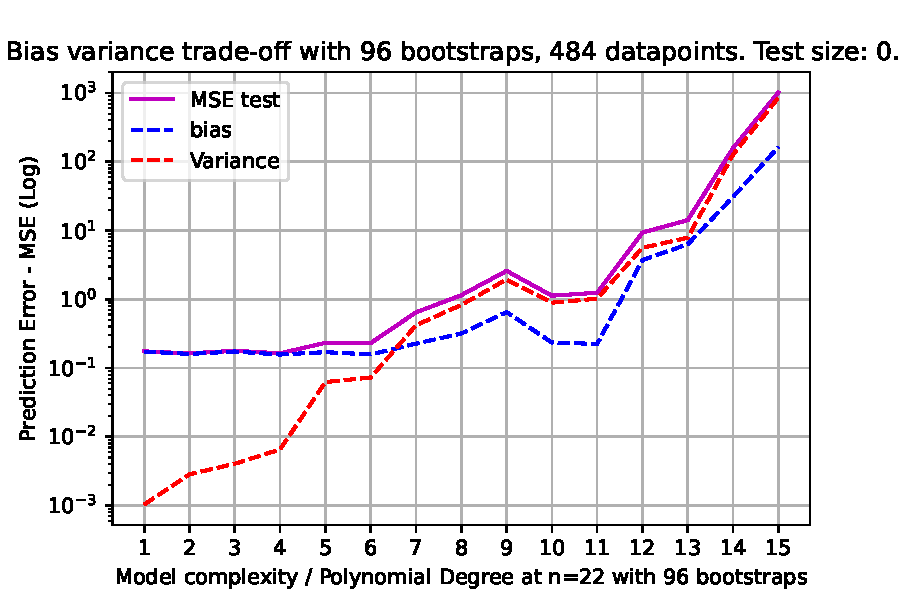
\includegraphics[width=\textwidth]{figures/EX2_model_complexity_using_bootstrap_function_n_22_testsize_0.3.pdf}
      \caption{400 datapoints, 200 bootstraps}
      \label{fig:bootstrap_bias_var_n_20}
  \end{subfigure}
  \hfill
  \begin{subfigure}{0.49\textwidth}
      \centering
      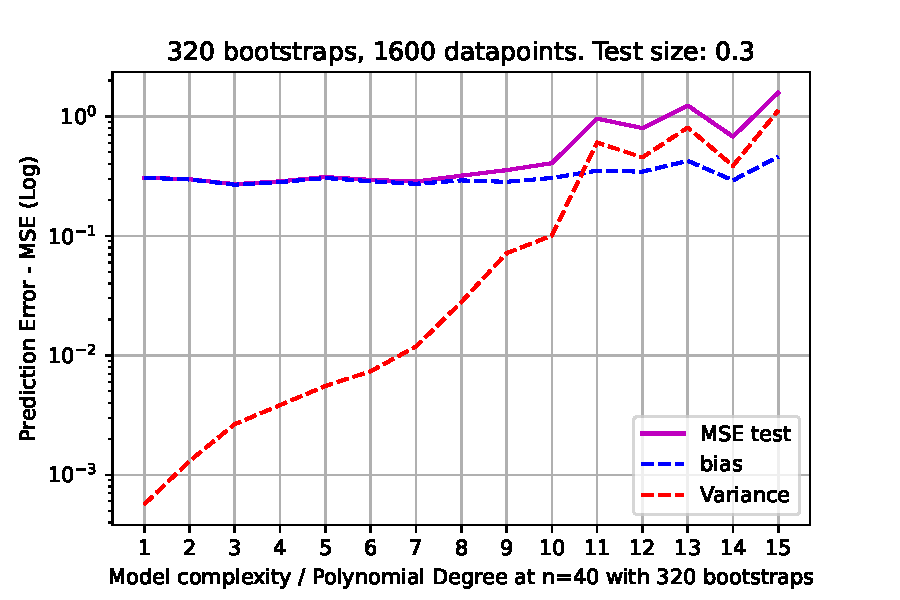
\includegraphics[width=\textwidth]{figures/EX2_model_complexity_using_bootstrap_function_n_40_testsize_0.3.pdf}
      \caption{1600 datapoints, 800 bootstraps}
      \label{fig:bootstrap_bias_var_n_30}
  \end{subfigure}

     \caption{Bias variance trade-off with bootstrap}
     \label{fig:bootstrap_bias_var}
\end{figure}




\section*{\label{ex:3}Exercise 3}
In the first part of this project, an infinite number of data points could easily be created by simply adjusting the number of \emph{n} decimals created in the span [0,1] for x and y. Setting \emph{n} to a large value could then, in turn, yield a data set of substantial size, which ables the prediction of estimated average test error with statistical certainty. However, for real-life purposes, this is rarely the case. More often than not, the challenges related to the validation of models in question lies in the limitations of available data. A potential pitfall in evaluating a model's performance is that the model might be biased towards specific data only contained in parts of the data. 

In the previous task, bootstrap was used to provide better estimates of a model's performance.  In this task, we will implement the cross-validation method to better measure the model's ability to generalize. 

This algorithm is implemented by dividing the dataset into K parts of roughly the same size. In this project, we try K values ranging from 5 to 10, which also coincides with best-practice values \cite{Hastie2009}.  We have implemented the split into K-folds by using the method K-fold from Scikit learn model-selection \cite{link_to_doc}. This method provides us with arrays of approximately equal size, consisting of indices for choosing test- and train data.  Each fold is then used once as a test set, while the remaining K-1 folds make up the training set. The overall purpose of this method is to produce an estimate of the prediction error, given by:

\[
  \text{CV}(\hat{f}) = \frac{1}{K}
  \sum_{i=1}^{K}L(y_i,\hat{f}^{-k(i)}(x_i))
\]

where $\hat{f}^{-k}(x)$ denotes the fitted function, in this case the linear regression model, with the \emph{k}th part of the data removed.\cite{Hastie2009}  

The following figures provide a visualizes the results of 5-10 fold cross-validation on a dataset consisting of a total of $22^2$ points\cite{notebook_exc3}. The MSE for polynomial degrees ranging from 3 to 14 is then calculated. Here we present the results from degrees 4 and 12, while the remaining is available in {.......}


The MSE estimated by bootstrap for the corresponding polynomial degree is also plotted. As figure ? displays,  at degree 4, the size of K seems to be of little importance, as the mean MSE of every fold is moderately low at approximately 0.10, with a standard deviation ranging from 0.8 to .012.

\begin{figure}[h]
  \centering
  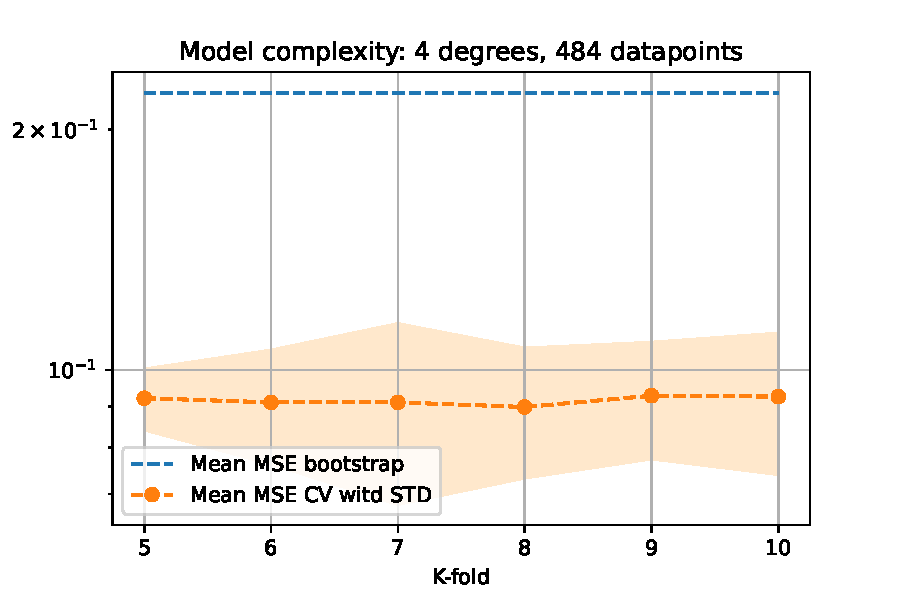
\includegraphics[scale=0.75]{figures/EX3_mse_cv_boot4.pdf}
  \caption{\label{fig:?} Mean MSE from CV and bootstrap at ploynomial degree = 4.}
\end{figure}



\begin{figure}[h]
  \centering
  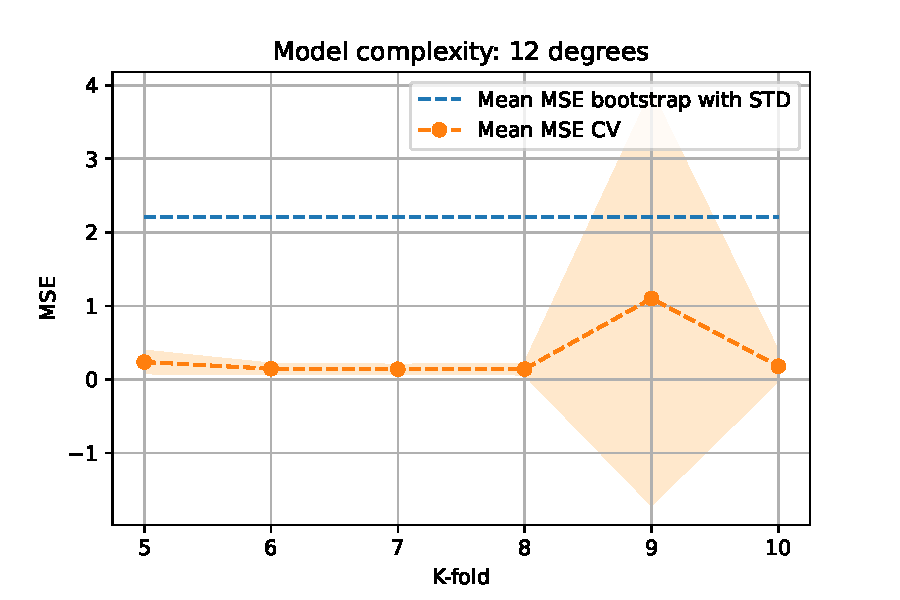
\includegraphics[scale=0.75]{figures/EX3_mse_cv_boot12.pdf}
  \caption{\label{fig:?}ean MSE from CV and bootstrap at ploynomial degree = 12.}
\end{figure}


However, when evaluating the results provided, it is of great importance to also assess the total size of the dataset as this could bias the estimate of error:

\subsection*{Comparing methods}


\todo[inline]{TODO: skriv mer om SKlearn comparison mot vår}
\begin{figure}[h]
  \centering
  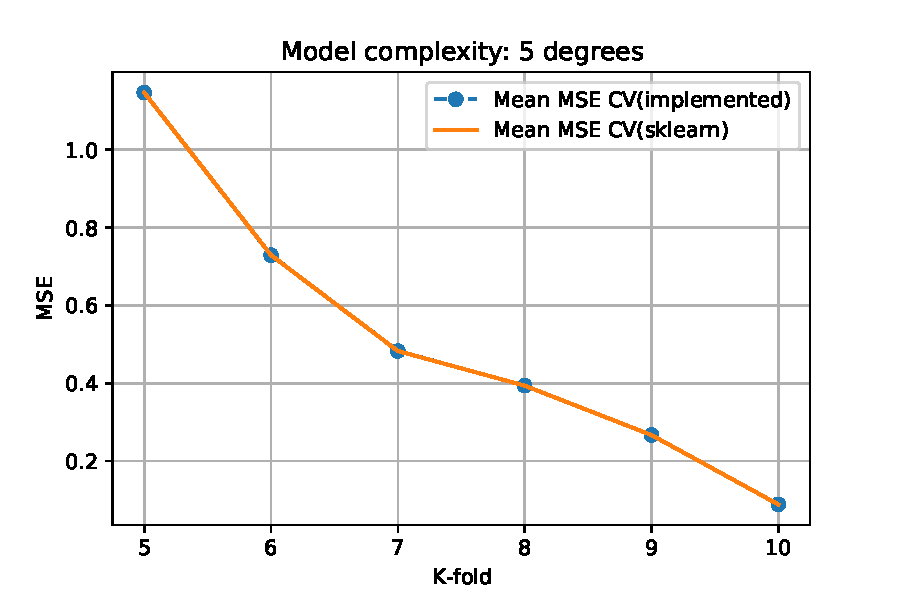
\includegraphics[scale=0.75]{figures/EX3_sk_vs_implemented_CV.pdf}
  \caption{\label{fig:?}Comparison of results from sklearn vs implemented method for Cross-Validation}
\end{figure}


The scores from Scikit-learn needed to be multiplied with $-1$ before beeing compared to our own results. This is due to the feact that this method expects a "greater is better" function rather than a cost function, resulting in an output opposite of the MSE.\cite{Geron2019} As illustrated by figure 8, we can conclude that our own implmented function produce the same results as the one fra Scikit-lean. As shuffeling is set to False as default in Scikit-learn, the same is done for our implmented method.





\section*{Exercise 4}
Throughout Exercise 1 - 3, we have studied function fitting using the Ordinary Least Squares regression. When comparing models, we have plotted the test error as a function of the model complexity and chosen a model based on the bias-variance tradeoff. The bias-variance tradeoff has also been studied in light of resampling techniques such as the bootstrap and k-fold cross-validation. As we have seen when interpreting the result of the resampling, an increased degree of freedom for the model will make the model more prone to overfit.

Instead of reducing the degree of freedom of a model by limiting it's order, we will in this section look at a different approach for model selection through the introduction of a regularization parameter $\lambda$. With the regularization parameter, individual predictors in the model can be restrained without resorting to reducing the overall order of the model. The regularization term will punish the predictors such that they stray from reaching large values, adding another method to control overfitting. \cite{Bishop2016}

Ridge regression is a regression model where the weights are constrained. \cite{Geron2019} This is done by adding a regularization term to the cost function, such that the function we are to optimize becomes
\[
  C\left(\bm{X},\bm{\beta}\right) = \left\{\left(\bm{y}-\bm{X}\bm{\beta}\right)^\text{T}\left(\bm{y}-\bm{X}\bm{\beta}\right)\right\}+\lambda\bm{\beta}^\text{T}\bm{\beta}
\]
Taking the derivatives of this function in terms of beta returns the closed form solution for the optimal $\bm{\beta}$
\[
  \bm{\hat{\beta}} = \left(\bm{X}^\text{T}\bm{X} + \bm{\lambda}\bm{I}\right)^{-1}\bm{X}^\text{T}\bm{y}
\]
As for Ordinary Least Squares regression, by using the closed form solution for the predictors we can predict new values $\tilde{y}$ as $\tilde{y} = \bm{X}\bm{\hat{\beta}}$.

\subsection*{The No Free Lunch Theorem}
As further motivation as to why we want to apply Ridge (and further on also Lasso) regression for fitting the Franke Function is due to the implications of the No Free Lunch Theorem. The theorem states that for any two learning models A and B, there are just as many situations where algorithm is A is superior to algorithm B as vice versa. \cite{Wolpert1996} The theorem implies that there are no sets of model that are guaranteed to fit a problem better than others. As a result of the theorem, regardless of the data being fitted, different models have to be individually evaluated for the given task at hand.

As there are no universally best learning algorithm for fitting the problem at hand, we expand our analysis of Fitting the Franke Function in light the No Free Lunch Theorem to also include an assessment of Ridge and Lasso Regression. Both models handles feature selection through the introduction of the regularization parameter lambda, thus potentially achieving a lower MSE than for Ordinary Least Squares. Introducing several models also follows the implications of the Free Lunch Theorem, notably that we have to fine tune and assess our models to perform well on the current problem. \cite{Goodfellow2016}

\subsection*{Weight Decay}
The Cost function for Ridge regression can be seen as the Cost function for Ordinary Least Squares with an added weight decay term $\lambda\bm{\beta}^\text{T}\bm{\beta}$. The parameter $\lambda$ is known as a hyperparameter, i.e. the parameter can be controlled before fitting the model and changes how the model behaves during fitting and predicting. \cite{Goodfellow2016} Moreover, $\lambda \geq 0$, such that $\lambda$ close to $0$ implies Ordinary Least Squares and $\lambda$ large implies that the predictors are close to $0$. Hence the term weight decay, as the hyperparamter can be tuned to enforce some predictors (weights) to gradually be excluded from the model fit.

For this Exercise, we will analyse the effect of the weight decay when fitting the Franke Function using Ridge regression. We will analyse the polynomial of optimal degree that we determined in the previous exercises through assessing the bias-variance tradeoff for an increased model complexity. Firstly with the bootstrap resampling technique, then compared the bootstrap MSE with what was obtained using the k-fold cross validation. With the model complexity

\subsection*{Implementing Ridge regression}
Our implementation of Ridge regression follow closely that of Ordinary Least Squares, but with an input parameter $\lambda$ determining the strength of the regularization term. Furthermore, the implementation differs as the normal equation for computing the optimal predictors have changed to $\bm{\hat{\beta}} = \left(\bm{X}^\text{T}\bm{X} + \bm{\lambda}\bm{I}\right)^{-1}\bm{X}^\text{T}\bm{y}$. When implementing Ridge regression, we follow the convention that the intercept is skipped when fitting the function, hence we start computing the regularization term starting at $\beta_1$. \cite{Geron2019} if the intercept were included, the regularizer would be dependant on the choice of origin for the target, which generally causes the mean squared error to increase as touched upon during the first Exercise.

\begin{figure}
  \centering
  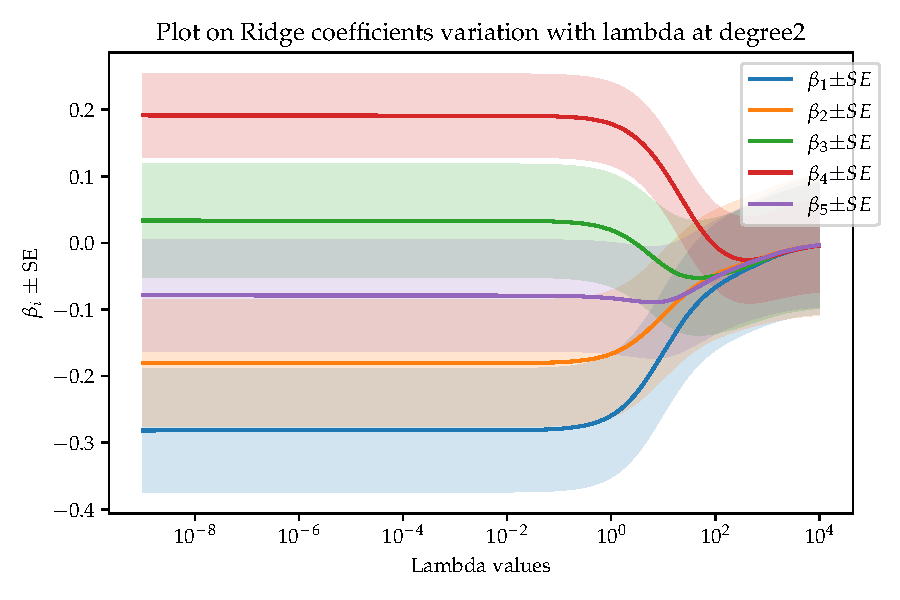
\includegraphics[scale=0.75]{figures/EX4_beta_plot_ridge_2.pdf}
  \caption{\label{fig:ridge_beta_1}Plot of the weight decay on the individual predictors for our Ridge regression with a second order polynomial}
\end{figure}

Figure (\ref{fig:ridge_beta_1}) shows the effect of the regularizer for a fitted model of order 2. The figure clearly shows the weight decay, as the individual predictors start off essentially unaffected, until they are gradually decayed to 0 at independent rates. additionally, following the weight decay plot, we can understand how the regularizer affects the final model fit as already mentioned in the previous section. The case of the regularization parameter $\lambda$ achieving larger values, which forces all predictors to become 0, would result in the fitted model being a flat plane centered around 0. Thus, to study where the regularization parameter would attain an optimal fit, we plot a Search Landscape over all degrees and lambda values.

\begin{figure}
  \centering
  \hspace*{-3.5cm}
  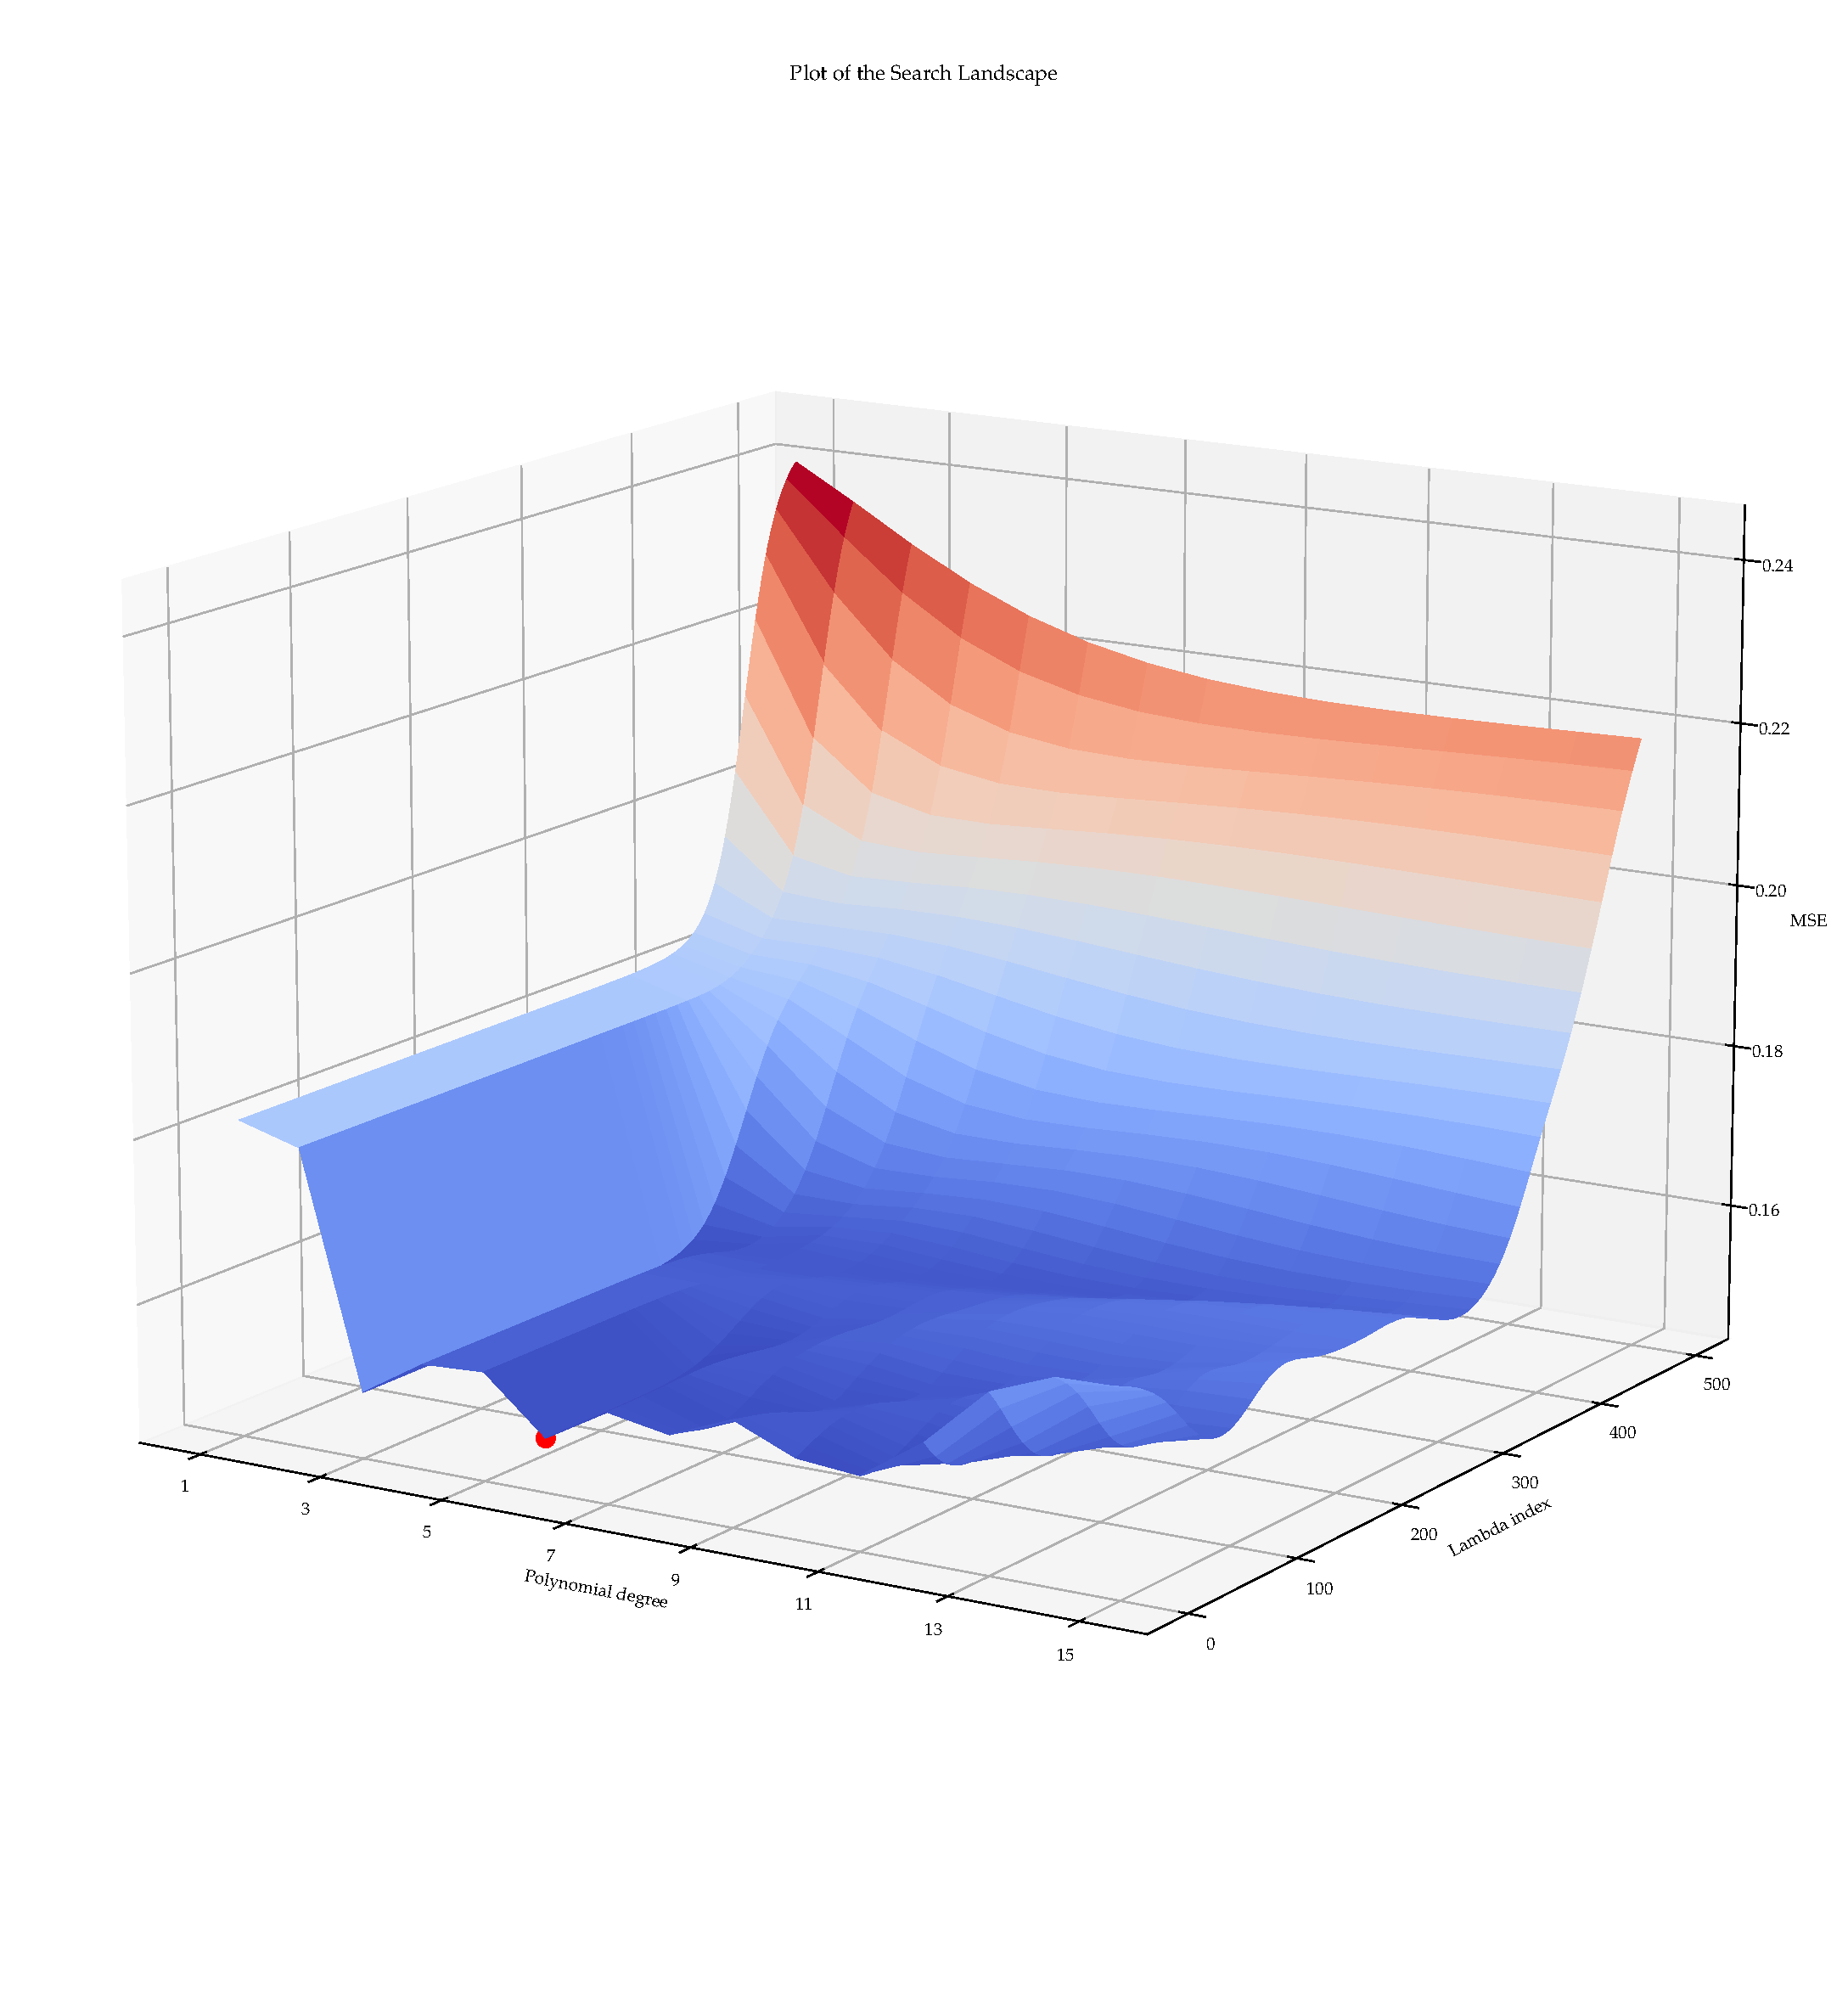
\includegraphics[scale=0.58]{figures/EX4_search_landscape_plt.pdf}
  \caption{\label{fig:ridge_search_land}Plot of the Search Landscape for polynomials up to a cretain order initialized with different regularization parameter values. The red dot symbolizes surface minimum.}
\end{figure}

The search landscape in Figure (\ref{fig:ridge_search_land}) gives us predicted MSE values for a Ridge polynomial of order up to 15. With regularization parameters on a range $\lambda \in \left[10^{-9},10^{4}\right]$ As such, we can use the search landscape to make an initial guess at where the optimal degree and regularization parameter combination will be based on where the lowest MSE is located. For our Ridge regression model, that initial guess would be degree 6, with a $\lambda = 10^{-9}$.

Though an initial guess at the optimal Ridge model has been made, we have to further study the model by applying the resampling techniques developed and explored in \nameref{ex:2} and \nameref{ex:3}.

\section*{Exercise 5}
The second regularized linear model which we will study is Least Absolute Shrinkage and Selection Operator (LASSO) Regression. Lasso adds a regularization term to the Cost function similarly to Ridge regression, though Lasso utilizes the L1 norm of the predictors instead of the L2 as in Ridge. \cite{Geron2019} Mathematically, adding the L1 regularizer gives us the following Cost function
\[
  C\left(\bm{X},\bm{\beta}\right) = \left\{\left(\bm{y}-\bm{X}\bm{\beta}\right)^\text{T}\left(\bm{y}-\bm{X}\bm{\beta}\right)\right\}+\lambda\lVert \bm{\beta}\rVert_1
\]
We note that the L1-norm is the same as the sum of the absolute value for each $\beta_i$. Moreover, the derivative of the absolute value is the sign-function. The resulting normal equation for Lasso regression is thus not a nice analytical expression, and is omitted for this Exercise. As a result, only the Sci-Kit implementation of Lasso regression will be studied.

\subsection*{Difference between L1 and L2-norm regularization}
The difference between the L1 and L2-norm is how it can be related to our understanding of distance. The L1-norm, mathematically defined as $\lVert \bm{\beta} \rVert_1 = \sum_{i=0}^{n-1}|\beta_i|$ is the "Manhattan Distance" of $\bm{\beta}$, i.e. the distance from two points a to b using only straight and normal lines. On the other hand, the L2-norm is mathematically defined as $\lVert \bm{\beta} \rVert_2 = \sqrt{\sum_{i=0}^{n-1}\beta_i^2}$. The L2-norm is more commonly referred to as the Euclidean distance, or the distance of a straight line drawn between a and b.


\section*{Exercise 6}
The main goal of exercise 6 is to analyze the performance of our models on real digital terrain data using the approach essentially conducted in previous exercises
1-5 except for bootstrap. The project text tells us to use cross-validation as resampling for model evaluation, and we interpret this such that we are not expected
to implement bootstrap at all. \\
Before commencing model evaluation and analysis in exercise 6, we had to understand the terrain data's nature, how it differs from the franke function data in 
complexity and how the terrain data is assembled to fit our models. Looking at the terrain data, it is rather complex comparing the relatively smooth shape of the 
franke function. The terrain landscape has several structures, shapes, and contours, while the frank function has only three smooth dominating structures in its landscape,
two Gaussian peaks together with one slight dip. For the synthetically created franke function data, we had to add noise in order for us to analyze the robustness of 
the models and to which degree the models were generalized. Controlling the influence and magnitude of the noise is a luxury situation, and for the real terrain image,
we do not know the noise. The noise in the terrain data is incorporated within the image itself and stems from sensors and the assembly or construction of the image.

\subsection*{The assembly of the terrain data}
To recap on the franke function; one must decide on the number of points for x and y at a specific range, construct a meshgrid of x and y, then z is created based on 
the franke function. For the franke function we randomly and uniformly chose $x,y$ such that $\forall x,y \in{[0.0,1.0]}$, where the number of points is equal for both
y and x. Comparing the franke function to the terrain data, we get the z variable from the terrain image itself. The values of the z variable in the terrain data represent 
height or depth similarly as for the franke function. However, the height or depth in the terrain data image represents the real height in the actual topographical terrain
having an entirely different scale comparing the constructed range between 0-1 of the franke function. Considering terrain data assembly for the x and y variables, 
it must be constructed as a meshgrid spanning the entire range of all x and y pixel positions within the terrain image. Since the range of x and y is determined by 
the span of pixel positions corresponding to the image width and height, we must scale both the x and y variables from the terrain data. The terrain input data utilized
has dimensions 3601x1801, inducing 6485401 data points for the entire dataset. Comparing the constructed franke function, the terrain image is not quadratic, meaning 
the range of x and y is not equal. Therefore, both the shape and values of the terrain data motivates to data scaling (both inputs and targets) to prevent one feature,
by its magnitude, from dominating over the other. 

\subsection*{Terrain data scaling and resize}
One must avoid the model to favor features by their magnitude since the contribution from features of smaller magnitude can be equally strong or important. 
Hence, the x-direction in real terrain is equally important as the y-direction even though the higher end of x is at 3600 and the higher end of y is at 1800. 
Therefore, we scale the terrain data using a standard scaler for the input and target data. It makes sense also to scale the target data since it represents 
height and dept in meters and scaling yields a uniform reference system, and it can also avoid numerical floating-point errors. Furthermore, considering the Lasso regression,
which uses gradient-based optimization, scaled targets make convergence a lot faster.  
Apart from scaling the data, another approach contributing to equalizing the importance of the x and y variable (features) in the terrain data is to resize the image into a
quadratic form where image height equals image width. However, resizing the entire image into a quadratic form will transform and distort the nature of the topographical 
terrain we try to fit. We tackled this by first resizing while keeping the scale factor between width and height to make the number of data points feasible to work with.
While keeping the terrain structures intact, we resized the image down to 10\% of its original size, figure \ref{fig:terrain_resized}. Moreover, we created 6x3 patches of
image data from the resized images where each patch being quadratic of dimension 60x60 (3600 data points), figure \ref{fig:terrain_patches}. We experimented with several 
different configurations of the grid size constituting all patches and the number of data points (pixels) within each patch regarding data complexity and terrain shape.
After investigating the different patches, we narrowed down to two patches, one from each terrain, figure \ref{fig:terrain_patches_focus}. We eventually decided to focus 
on patch2 from terrain1 since it yields both an interesting shape and is complex while not being infeasible to work with considering the models prone to the task. 
This preprocessing serves the purpose of feeding the model with only one patch, making a smaller subproblem that is more digestible for the model in the pursuit of a good 
fit on exciting data.\\
The motivation behind image resizing and resampling is not just to reduce the number of data points; it also relates to the closeness between data points. 
Having many similar data points may lead to biased model performance and that the model is not generalized properly. By resizing and resampling pixels from an image 
into a new smaller image with fewer pixels, the pixels in the smaller image have longer distances to each other.
\begin{figure}
  \centering
  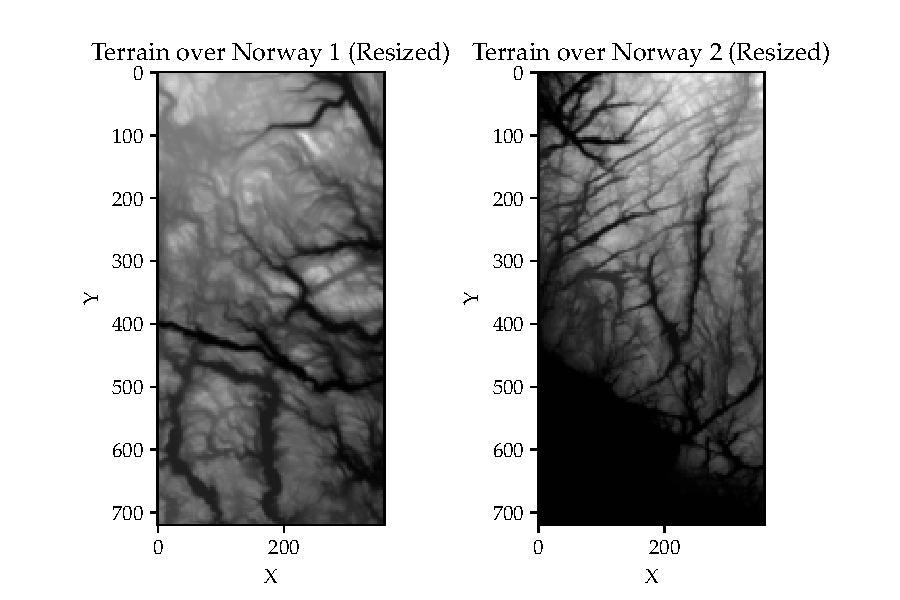
\includegraphics[scale=0.75]{figures/EX6_terrain_data_resized.pdf}
  \caption{Terrain data resized}
  \label{fig:terrain_resized}
\end{figure}
\begin{figure}
  \centering
  \subfloat{{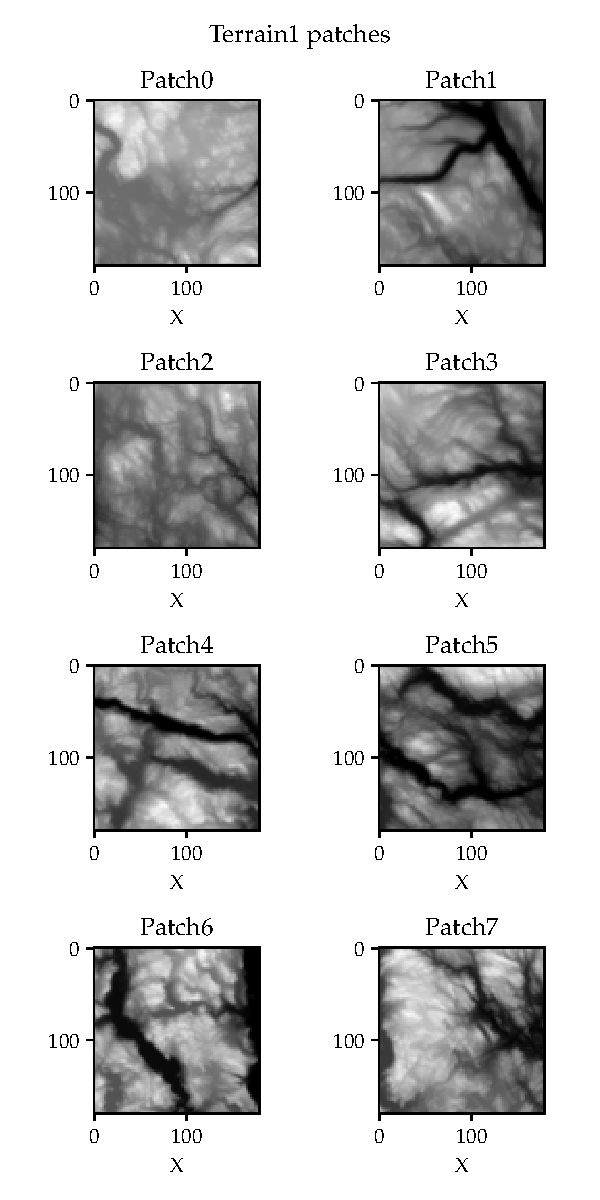
\includegraphics[width=7cm]{figures/EX6_Terrain1 patches.pdf} }}%
  \subfloat{{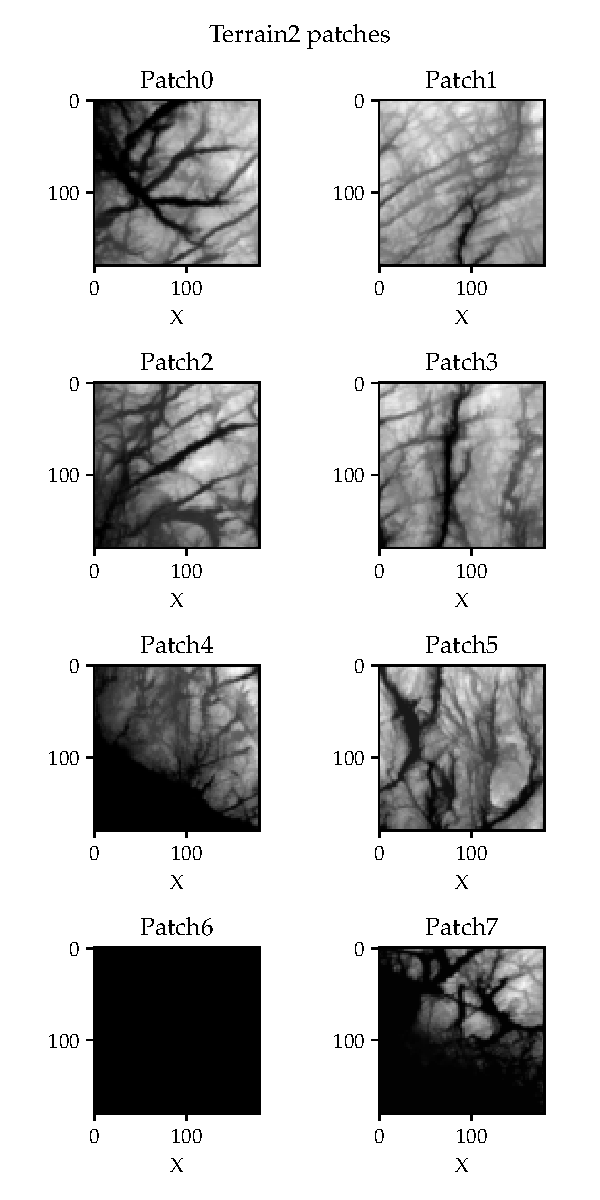
\includegraphics[width=7cm]{figures/EX6_Terrain2 patches.pdf} }}%
  \caption{Terrain patches}%
  \label{fig:terrain_patches}%
\end{figure}
\begin{figure}
  \centering
  \subfloat{{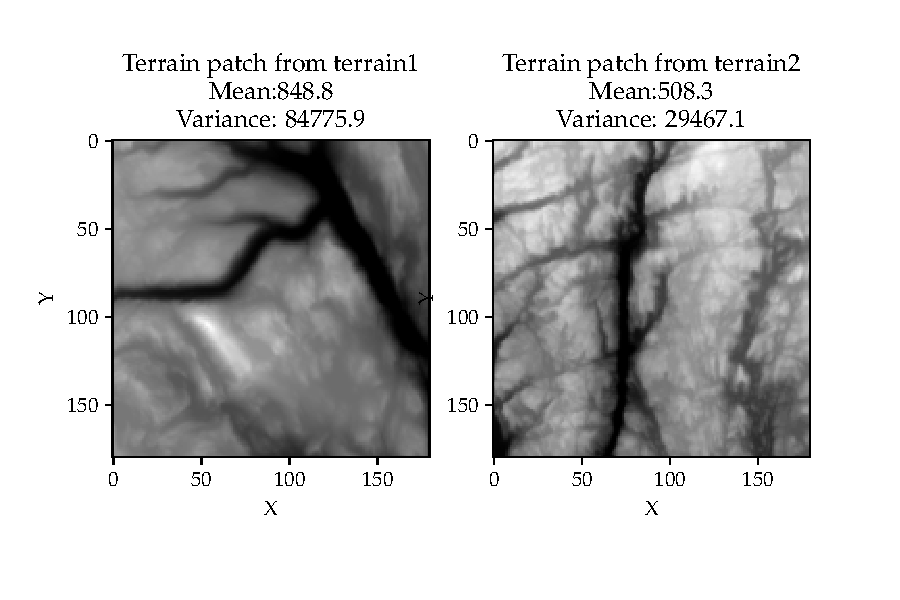
\includegraphics[width=14cm]{figures/EX6_terrain_patch_to_fit_2D.pdf} }}%
  \\
  \subfloat{{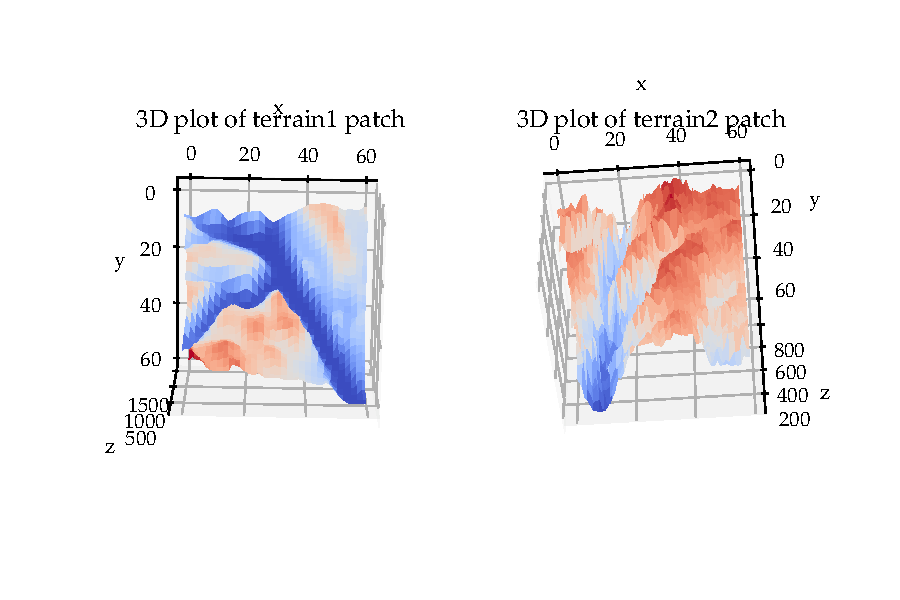
\includegraphics[width=15cm]{figures/EX6_terrain_patch_to_fit_3D.pdf} }}%
  \caption{Chosen terrain patches}%
  \label{fig:terrain_patches_focus}%
\end{figure}

\subsection*{Example}
For simplicity, let’s consider the image of size 7x7 
with 49 data points (pixels) drawn in figure\ref{fig:image_resizing}. Let's assume you performed a train test split on the 7x7 image resulting in $\{x_0,x_1,x_7,x_8\}$ being contained in the 
training set. Let's assume each pixel value and its $(x,y)$ position counts as the distance of 1, then the Euclidean distance between $x_0$ and its nearest neighbors ($x_1$ and $x_7$) is both 1. 
The distance between $x_0$ and $x_8$ would then be $\sqrt{2}=1.41$.
\todo[inline]{ADD eclaedan dinstance formula with the values?}
Three similar pixel values are not much, but this is just an example highlighting the concept, and in real situations you basically get several pixels of very similar values in your training data. 
You can also end up having several pixels in the training set and the test set that are basically equal. It is not ideal to have datapoint in the trainin set and test set that represents the same data point value. 
Let’s say you resize the 7x7 image down to a 3x3 image by sampling 9 pixels from the original image of 7x7, as illustrated in figure \ref{fig:image_resizing}. Considering the resampled 3x3 image,
the Euclidean distance between one pixel and its nearest neighbors is not 1 anymore. The distance between pixel (y=0,x=0) and its nearest neighbor (y=0,x=1) and (y=1,x=0) 
in the 3x3 image is now the Euclidean distance between pixel $x_0$ and $x_3$, and $x_0$ and $x_{21}$ from the original image. Therefore, picking pixels from the 3x3 image for the training
set and the test set now results in data points within the training set and the test set not being considerably similar anymore. It also reduces the share of similar data 
points ending up in both the training and test sets, which is important. Having many data points in the test set that are similar to the training set makes it harder to 
determine overfitting since you basically test on many data points that are close to what the model has been trained on.
\begin{figure}
  \centering
  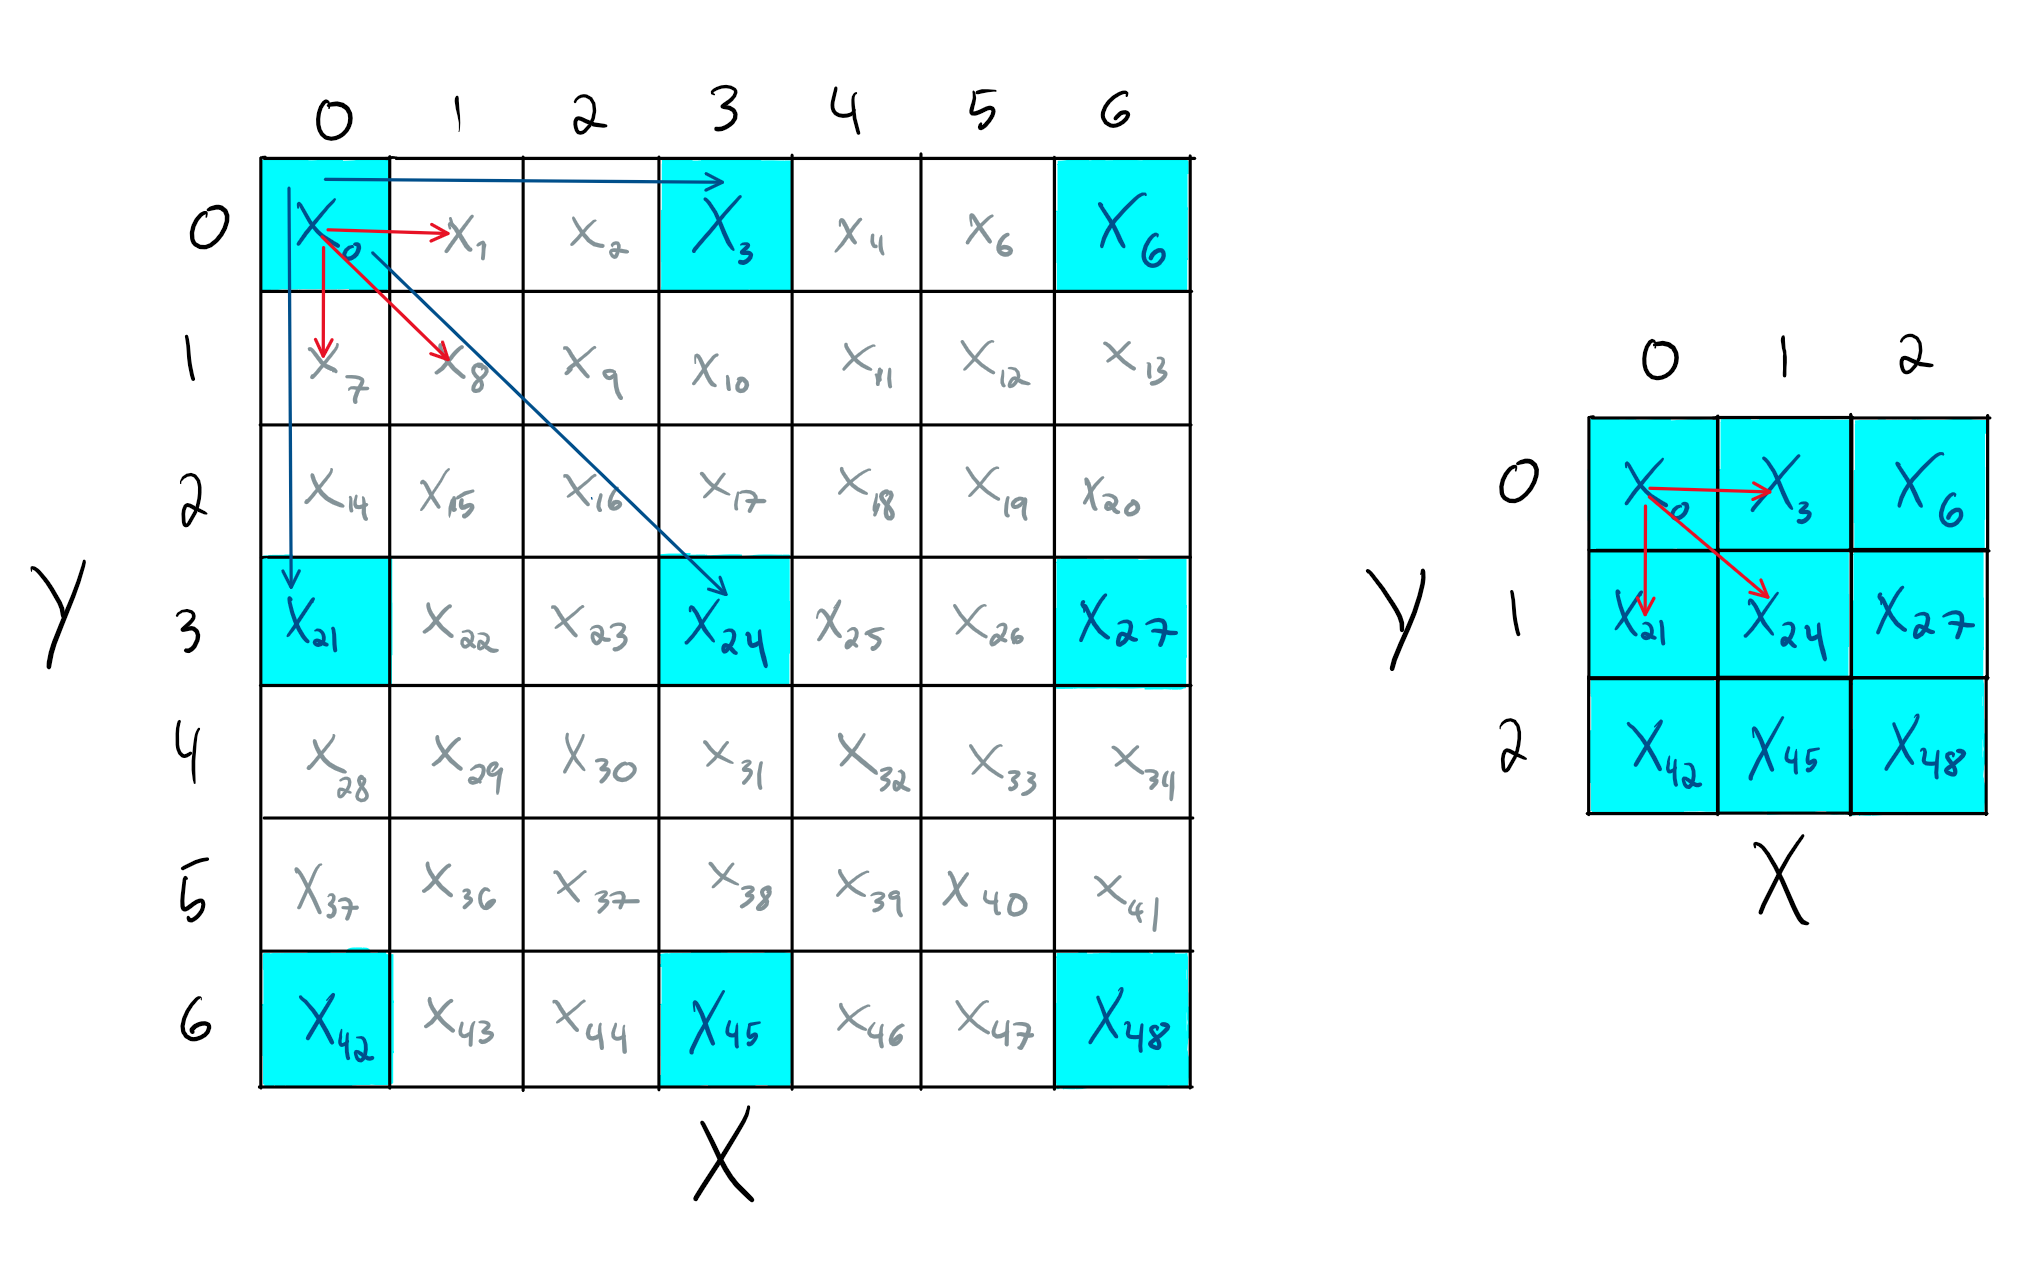
\includegraphics[scale=0.28]{figures/EX6_resizing.png}
  \caption{Distance between data points}
  \label{fig:image_resizing}
\end{figure}

\newpage
\subsection*{Exercise 6 - Conclusion and critical model selelction}
\subsubsection*{OLS fit}
\todo[inline]{TODO: Include bias-variance trade-off, fix figure references, include beta plots and compare between degree 10,11 and 12 to determain overfitting}
In this task we conducted a OLS fit on the the terrain1 patch using similar appraoch as done in exercise1. We fitted the OLS model between degree 1-44.
When approximating polynomials, the simpler components are often incorporated within the first coefficients of a model. The simpler components of an approximation 
often carry basic but significantly important information. When tackling the approximation of complex data, more coefficients must contribute in order to capture the 
real data's details, shape, and statistics. However, in approximation, the differences between degrees of complexity are not necessarily linear as it depends on the 
function that we want to approximate. Building on this, we generally expected our models to reach high complexity before running into overfitting relative to the data 
complexity for a particular terrain patch and the patch data size. Furthermore, we expected the training evaluation to indicate a minimum for the test MSE followed by a
certain plateau before major overfitting occurred for a reasonably complex terrain patch. 
We first experimented using terrain patches of 180x180 and observed that our models eventually reached a plateau for several degrees before slowly moving into overfitting.
A plateau of the test MSE most likely means that the difference from one degree to the next is not significant when capturing fine-grained details in the approximation.
Moreover, we changed the patch data size to 60x60 for easier analyses of model performance while still having exciting results and plots to investigate. 
In Figure \ref{fig:EX6_1_OLS_fit} the OLS model reaches the lower test MSE area at degree 10. The figure \ref{fig:EX6_1_OLS_fit} shows a plateau between degrees 10-14 before a clear sign of overfitting occurs, 
looking at the test MSE values. Looking at the R2 values, the R2 score on train and test are clearly taking different paths after degree 14, and from here on, 
the variation in the training data is increasingly described while the variation within the test data is decreasingly described. This is also a sign of overfitting since
the more variation described of the training data, the more you are fitted to the training data. However, just looking at test MSE and R2 scores is not always sufficient
to determine overfitting and to validate the robustness of the model and to which degree it is generalized. Just by looking at figure \ref{fig:EX6_1_OLS_fit}, we can have a range of degrees 
between degrees 9-14 which are candidates to be the most optimal degree. We consider the most optimal degree being a model that has consistent good performance and not being underfitted or overfitted. 
Looking at the CV plots in figure \ref{fig:EX6_1_CV}, degree 9 has a overall higher MSE score for the test data for all tested K-folds comparing the other degrees. Degree 9 also has a larger standard deviation 
in generall comparing the other degrees. The lower part of the standard deviation for degree 9 does not look to overlap into the other degrees for the majority of all K-folds. While it may not be so common 
to consider several K-folds when analyzing MSE and how well the model generalise to the data we took the liberty of of just doing that. We considered compariong models using all folds a reasonable task 
computational wise for all different degrees on the data size that we ended up using. We also though that given the relativly similar performance of degree 10, 11, and 12, it was an interesting task to 
look deeper to determain how consistent the model robustness is. Rounding up the analysis for degree 9, we also see that degree 9 is not as sharp as degree 10 looking at the predicted 2D terrain in figure \ref{fig:EX6_1_OLS_2D}. 
This excludes degree 9 as a candidate in the contest of being the moste optimal degree. 

Looking further in the CV plots in figure \ref{fig:EX6_1_CV}, degree 10,11, and 12 are relatively equal considering MSE for several K-folds. Looking at the standard deviation,
the robustness and generalization using these degrees seem to be reasonably equal given the slight differences between the degrees. To be fair, it looks that degree 11, the green color in the figure,
is haveing a smaller standard deviation and MSE for the majority of K-folds, and based on this; degree 11 takes the lead over degree 10 and 12. However, the standard deviation is overlapping for all 
degrees; 10, 11 and 12, meaning degree 11 may not better by statistically meassures. It is not easy to distinguish between degree 10,11 and 12 in the 
plots of the $\beta$ coefficients in the figures \ref{fig:EX6_1_OLS_betas_plot_degree10}, \ref{fig:EX6_1_OLS_betas_plot_degree11}, and \ref{fig:EX6_1_OLS_betas_plot_degree12} either. 
Many coefficentes with high standard errors can be a sign of overfit, but the all degrees appear relatively equal and does not show signs of a clear overfit. 

First when we study in detail the predicted product in the 3D plot and especially the 2D plots in figure \ref{fig:EX6_1_OLS_3D} and \ref{fig:EX6_1_OLS_2D}, we see important differences between the degrees. 
Degree 10 seems to have a smooth surface, while some unnatural artifacts are present at degrees 11 and 12 in the lower and right parts of the terrain images. We discovered that the predicted image gets artifacts and becomes more distorted at even higher degrees. 
This concludes that the artifacts and the distortions in predicted terrain images are indications of overfitting, leaving us with degree 10 as the most optimal degree. In general, you also want to have 
the simples possible model complexity which also favors degree 10 over degree 11 and 12. 
Another interesting observation we discovered is that the mean statistics of the predicted terrain image were correctly approximated at an early polynomial degree while the pixel variance differed more between degrees. 
The mean statistics of the approximated image are incorporated within the lower degrees and lower term coefficients, while the image variance is more aligned with the level of data and model complexity. 
This makes sense since image variance reflects the topographical variance within the real terrain we try to approximate. The more the terrain varies, the more complex the polynomial approximation. 
A lesson learned from this is to be critical to draw conclusions just by evaluating the MSE values, standard deviations and beta coefficients. It may be that you in the end have to 
evaluate to produced end product to be certain of which complexity that yields the best fit. 
\\\\
Based on the analyzis we conclude that degree 10 yeilds the best fit for the OLS model having a mean test MSE value of 0.169 and a standard deviation of 0.0075.
\\\\
Another intersting observation we though of mentioning is that our models are actualy performing as a type of image or data compression, where the model coefficients contain the information of considerably large terrain data. 

\subsubsection*{Ridge fit}
\todo[inline]{TODO: Ridge conclusion and critical model selelction. Write similar story as done for OLS using surfaceplon}
\subsubsection*{Lasso fit}
\todo[inline]{TODO: Lasso conclusion and critical model selelction. Write similar as done for Ridge}




\begin{figure}
  \centering
  \hspace*{-2cm}
  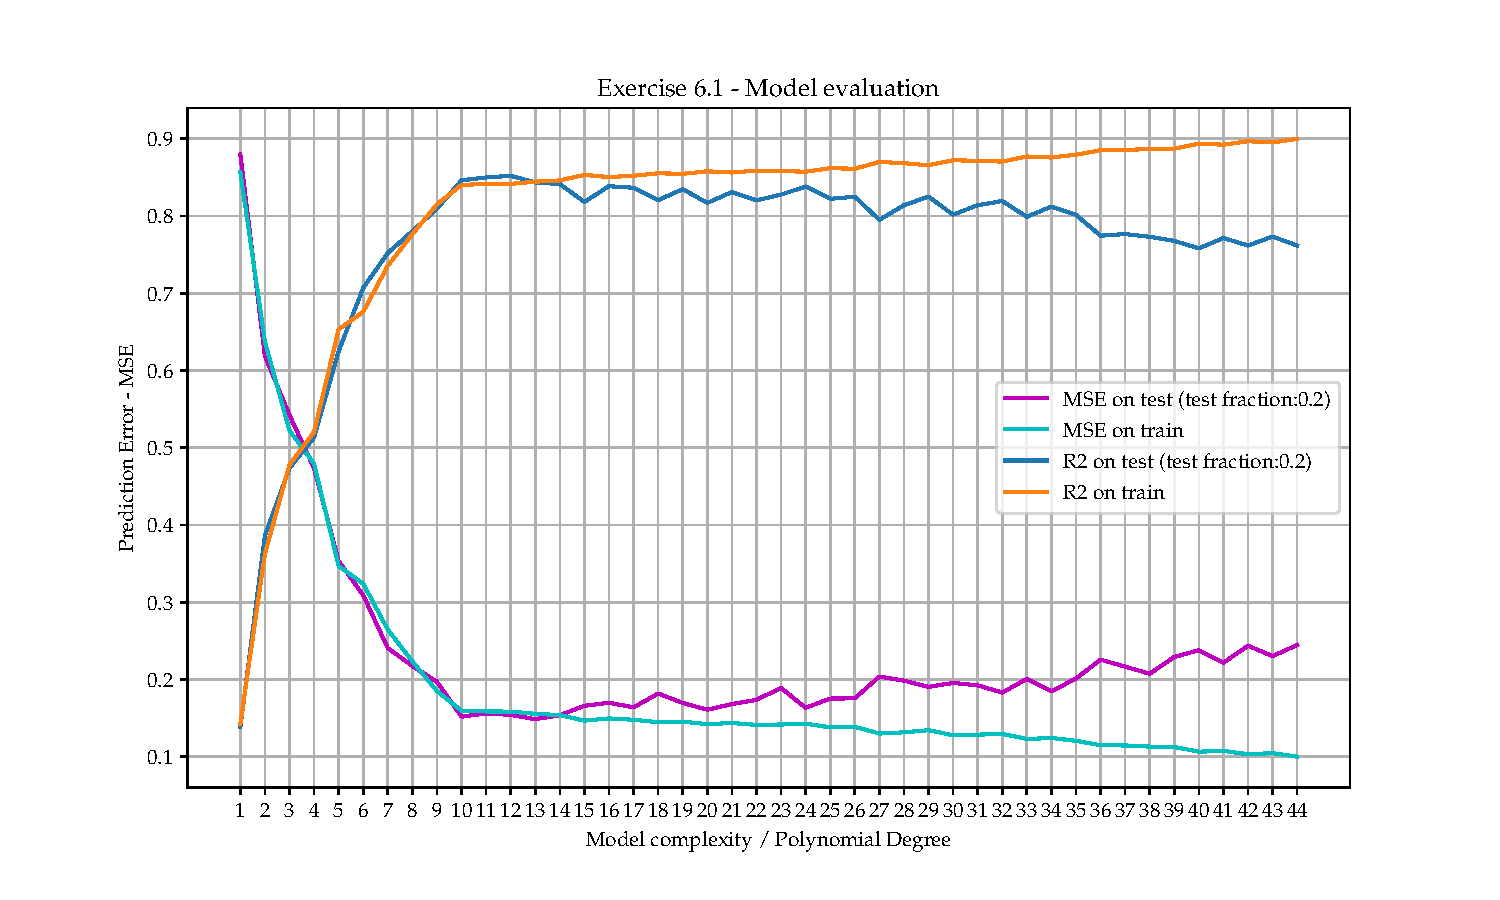
\includegraphics[scale=0.75]{figures/EX6_EX1_OLS_evaluattion.pdf}
  \caption{Model complexity vs prediction error using OLS}
  \label{fig:EX6_1_OLS_fit}
\end{figure}

\begin{figure}
  \centering
  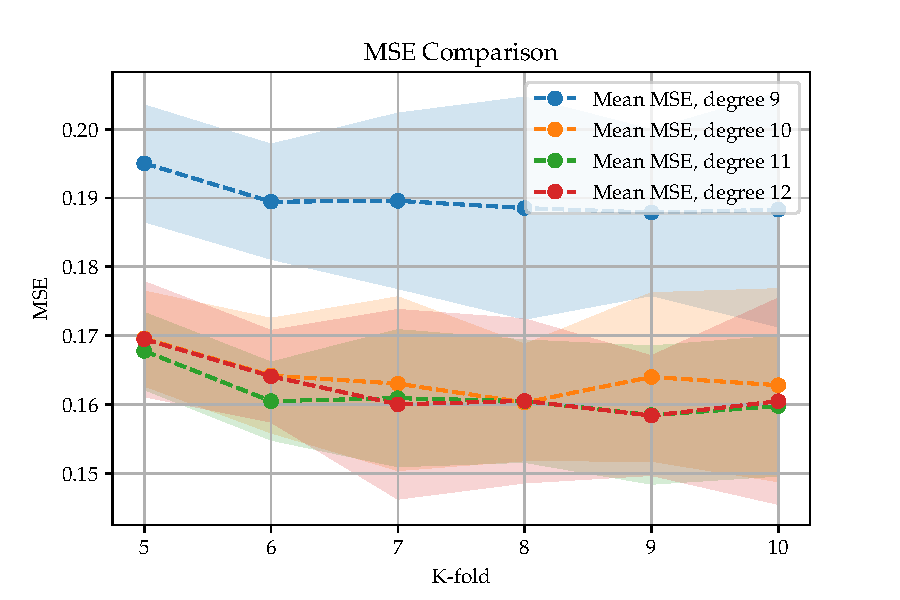
\includegraphics[scale=1.0]{figures/EX6_mse_cv_fold_compare_degrees.pdf}
  \caption{Cross-validation comparison for degree 9,10,11,12}
  \label{fig:EX6_1_CV}
\end{figure}

% \begin{table}
%   \centering
%   \csvautobooktabular{data/report_data/EX6_EX1_OLS_beta_error_degree5.csv}
%   \caption{Coefficient summary of OLS fit}
%   \label{data:EX6_1_OLS_betas}
% \end{table}

\begin{figure}
  \centering
  \hspace*{-4.2cm}  
  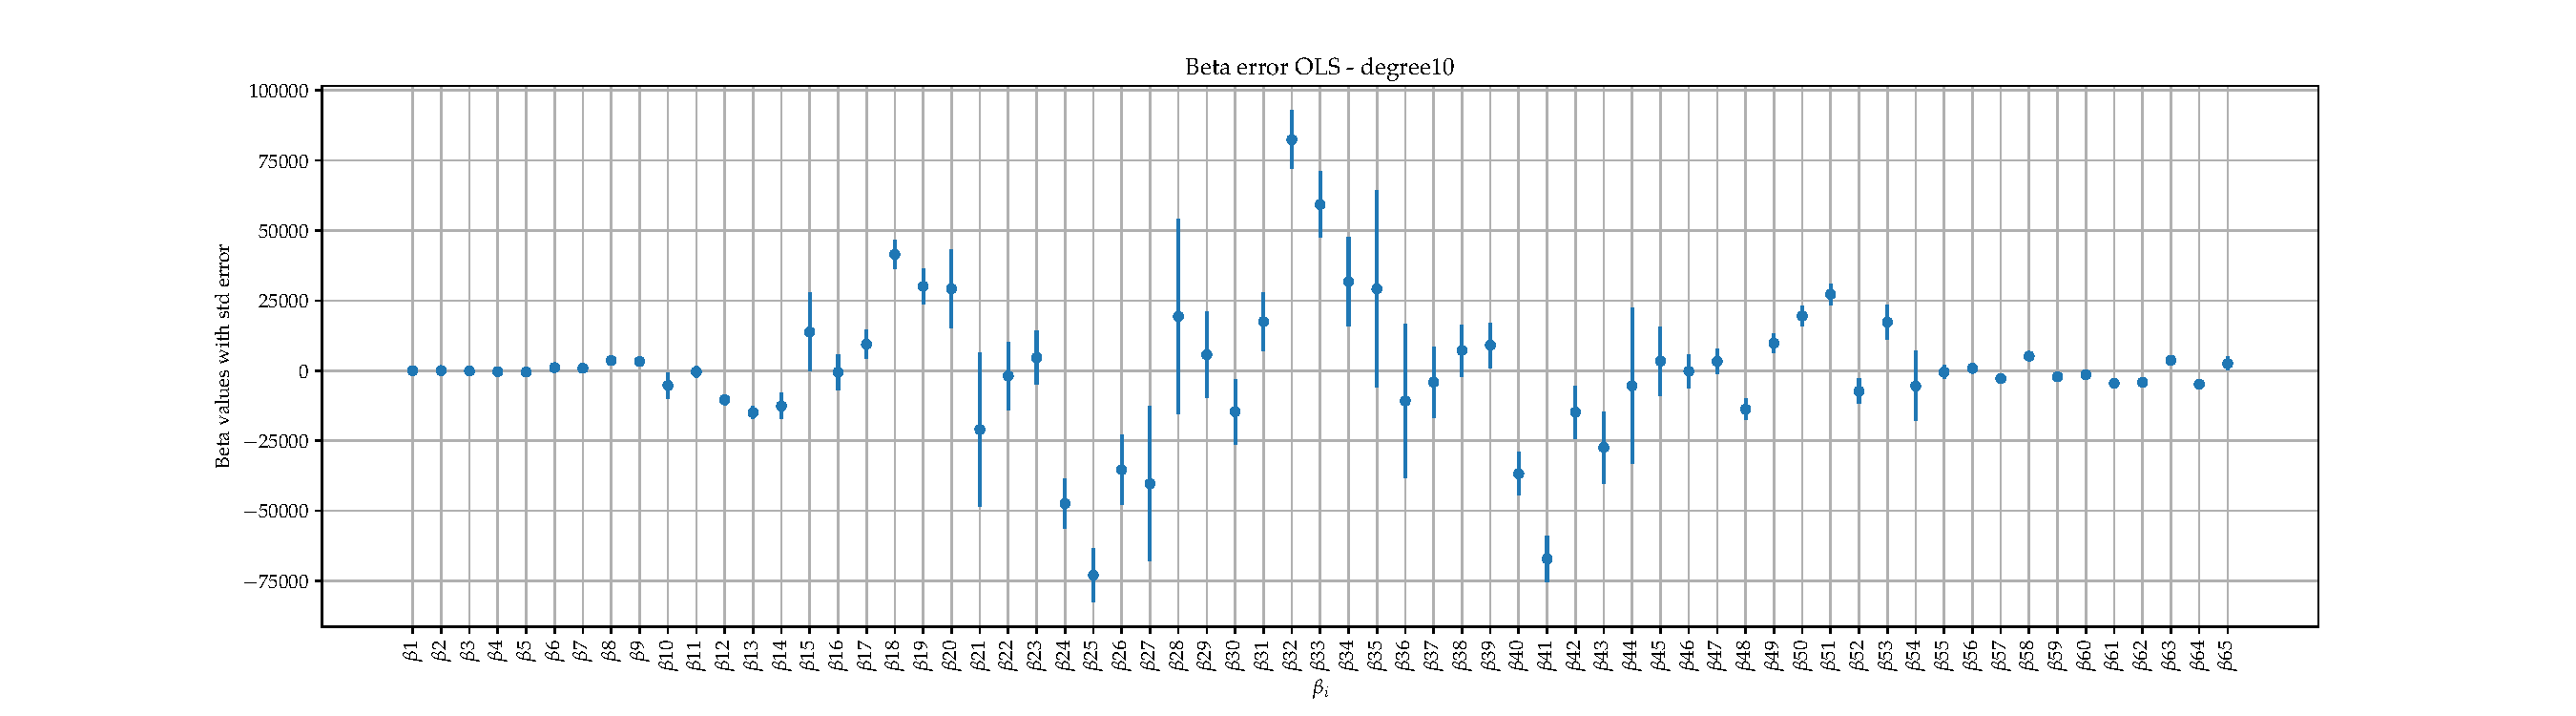
\includegraphics[scale=0.52]{figures/EX6_EX1_OLS_beta_error_degree10.pdf}
  \caption{Coefficients plot for degree 10}
  \label{fig:EX6_1_OLS_betas_plot_degree10}
\end{figure}

\begin{figure}
  \centering
  \hspace*{-4.2cm}  
  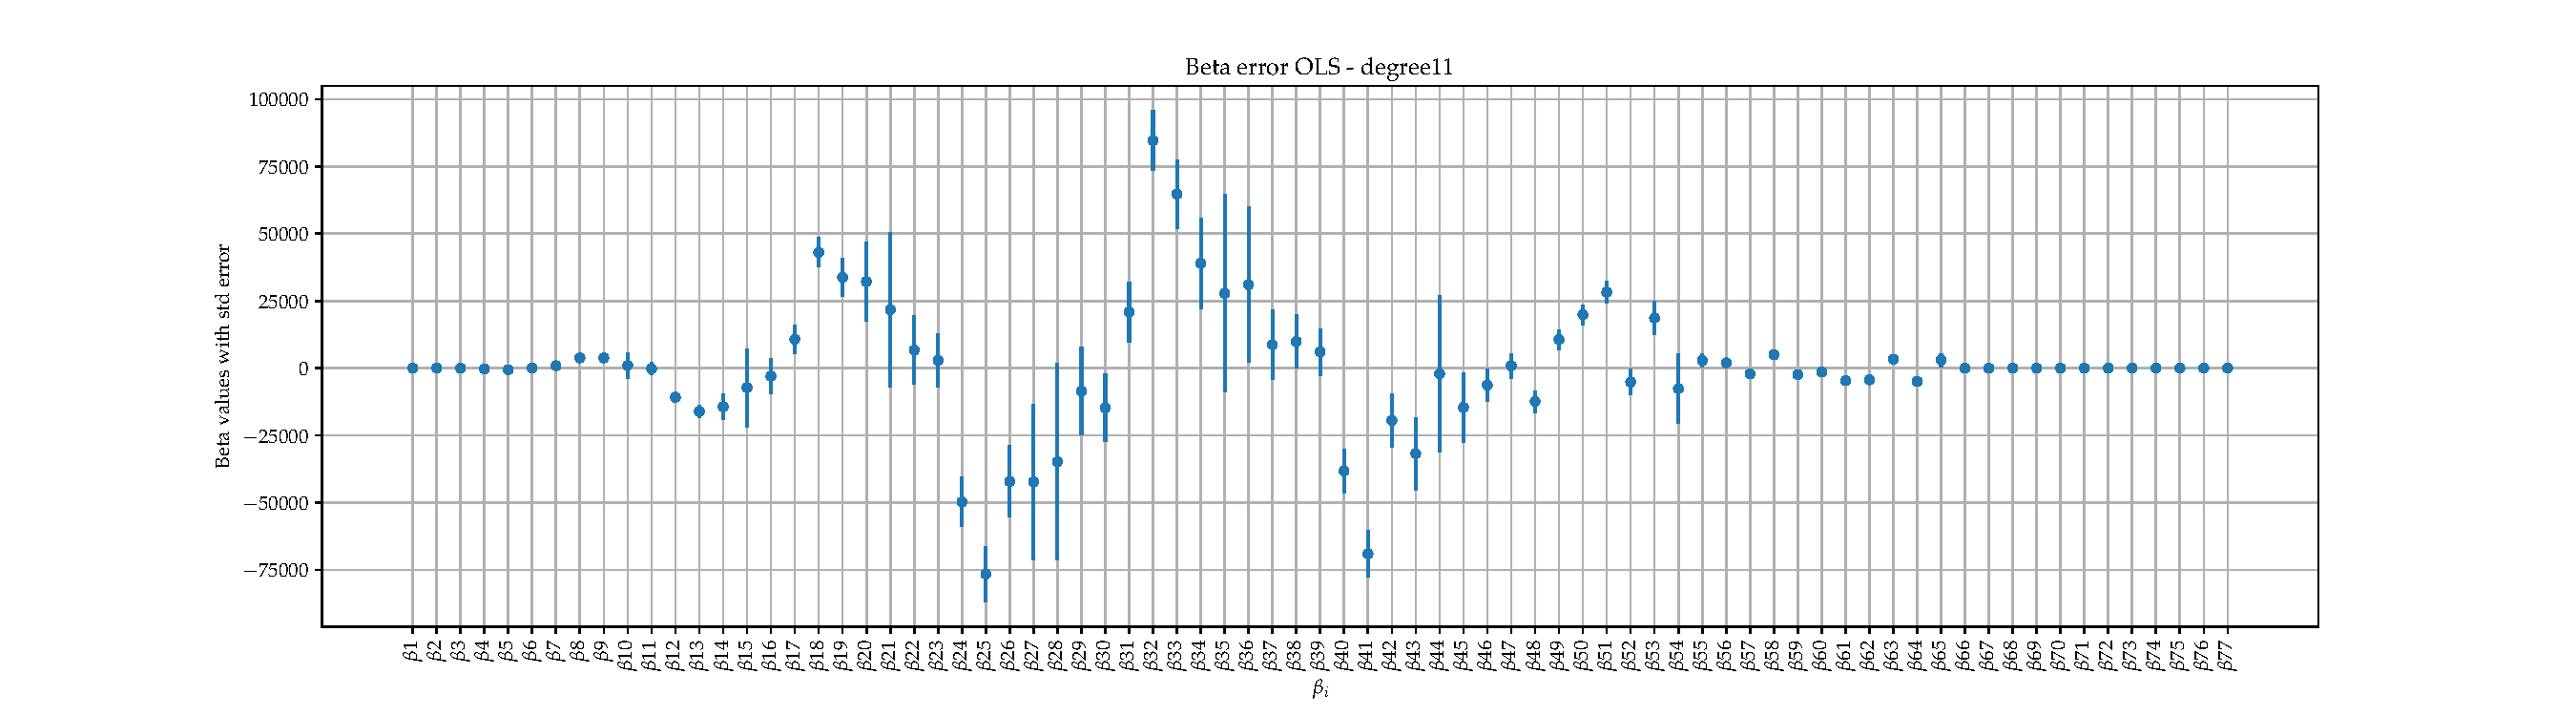
\includegraphics[scale=0.52]{figures/EX6_EX1_OLS_beta_error_degree11.pdf}
  \caption{Coefficients plot for degree 11}
  \label{fig:EX6_1_OLS_betas_plot_degree11}
\end{figure}

\begin{figure}
  \centering
  \hspace*{-4.2cm}  
  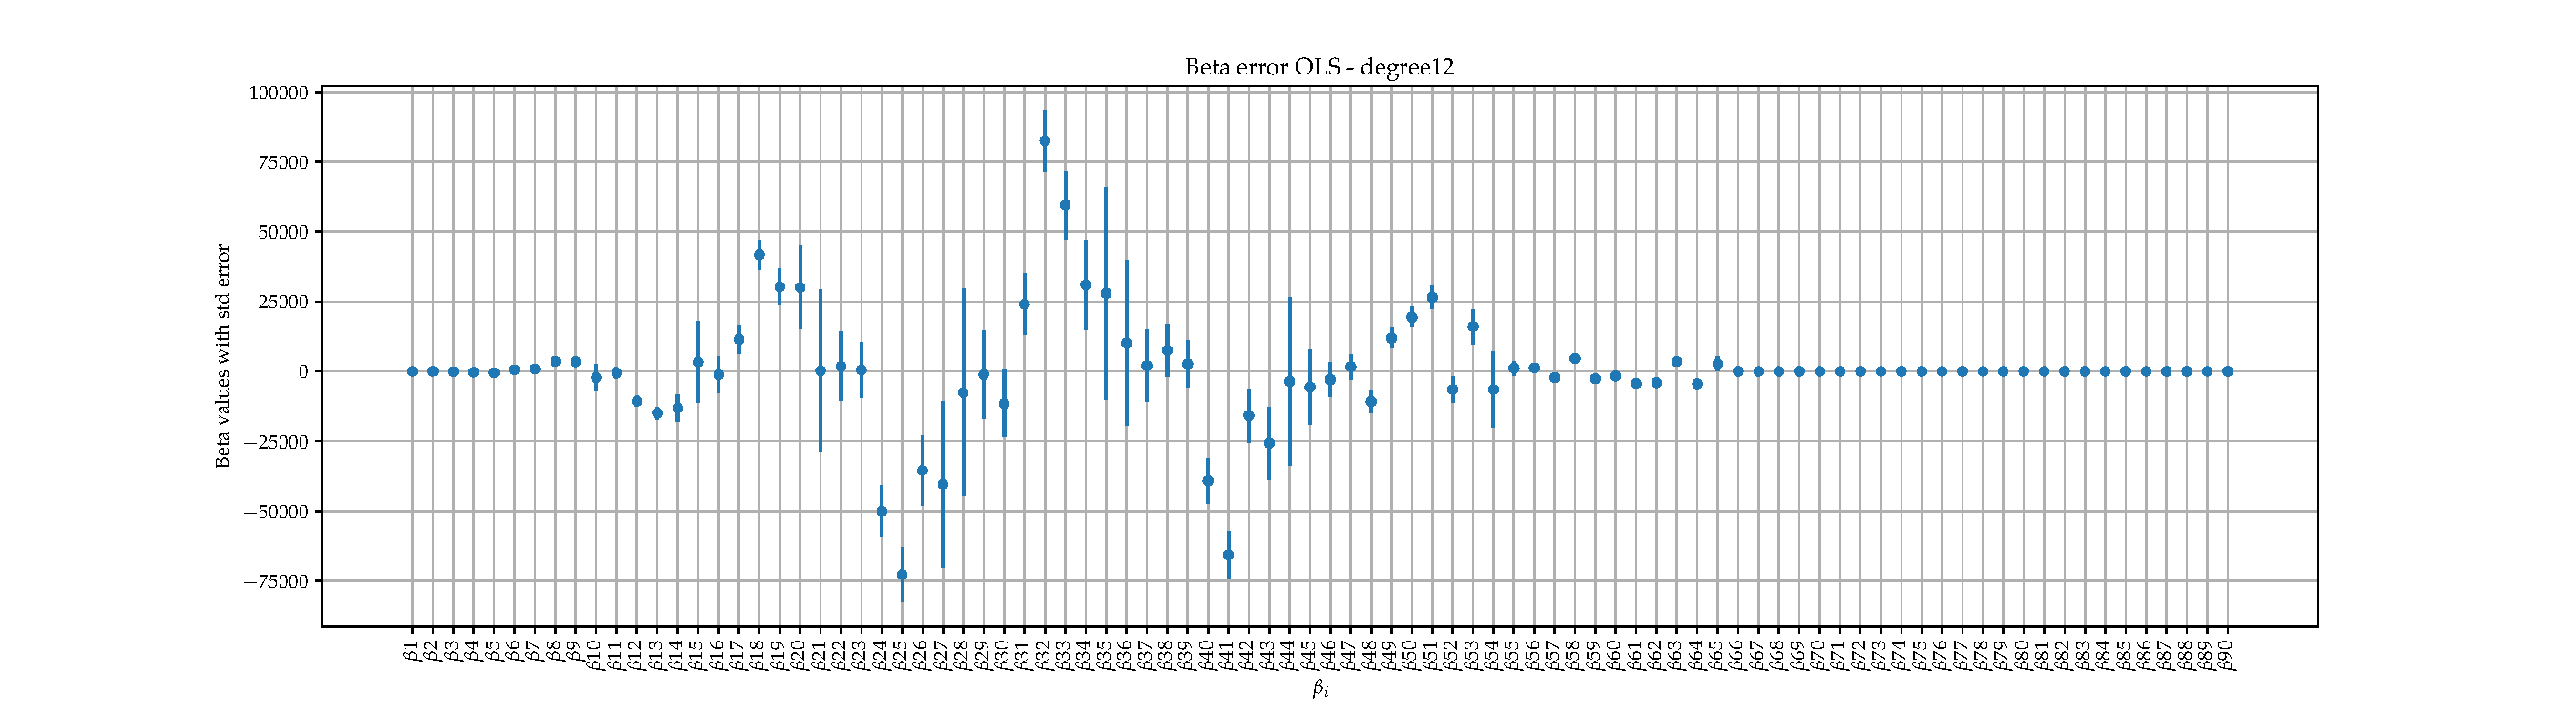
\includegraphics[scale=0.52]{figures/EX6_EX1_OLS_beta_error_degree12.pdf}
  \caption{Coefficients plot for degree 12}
  \label{fig:EX6_1_OLS_betas_plot_degree12}
\end{figure}


\begin{figure}
  \centering
  \caption{2D plot showing the produced product from models at degree9-12}
  \hspace*{-1.2cm}  
  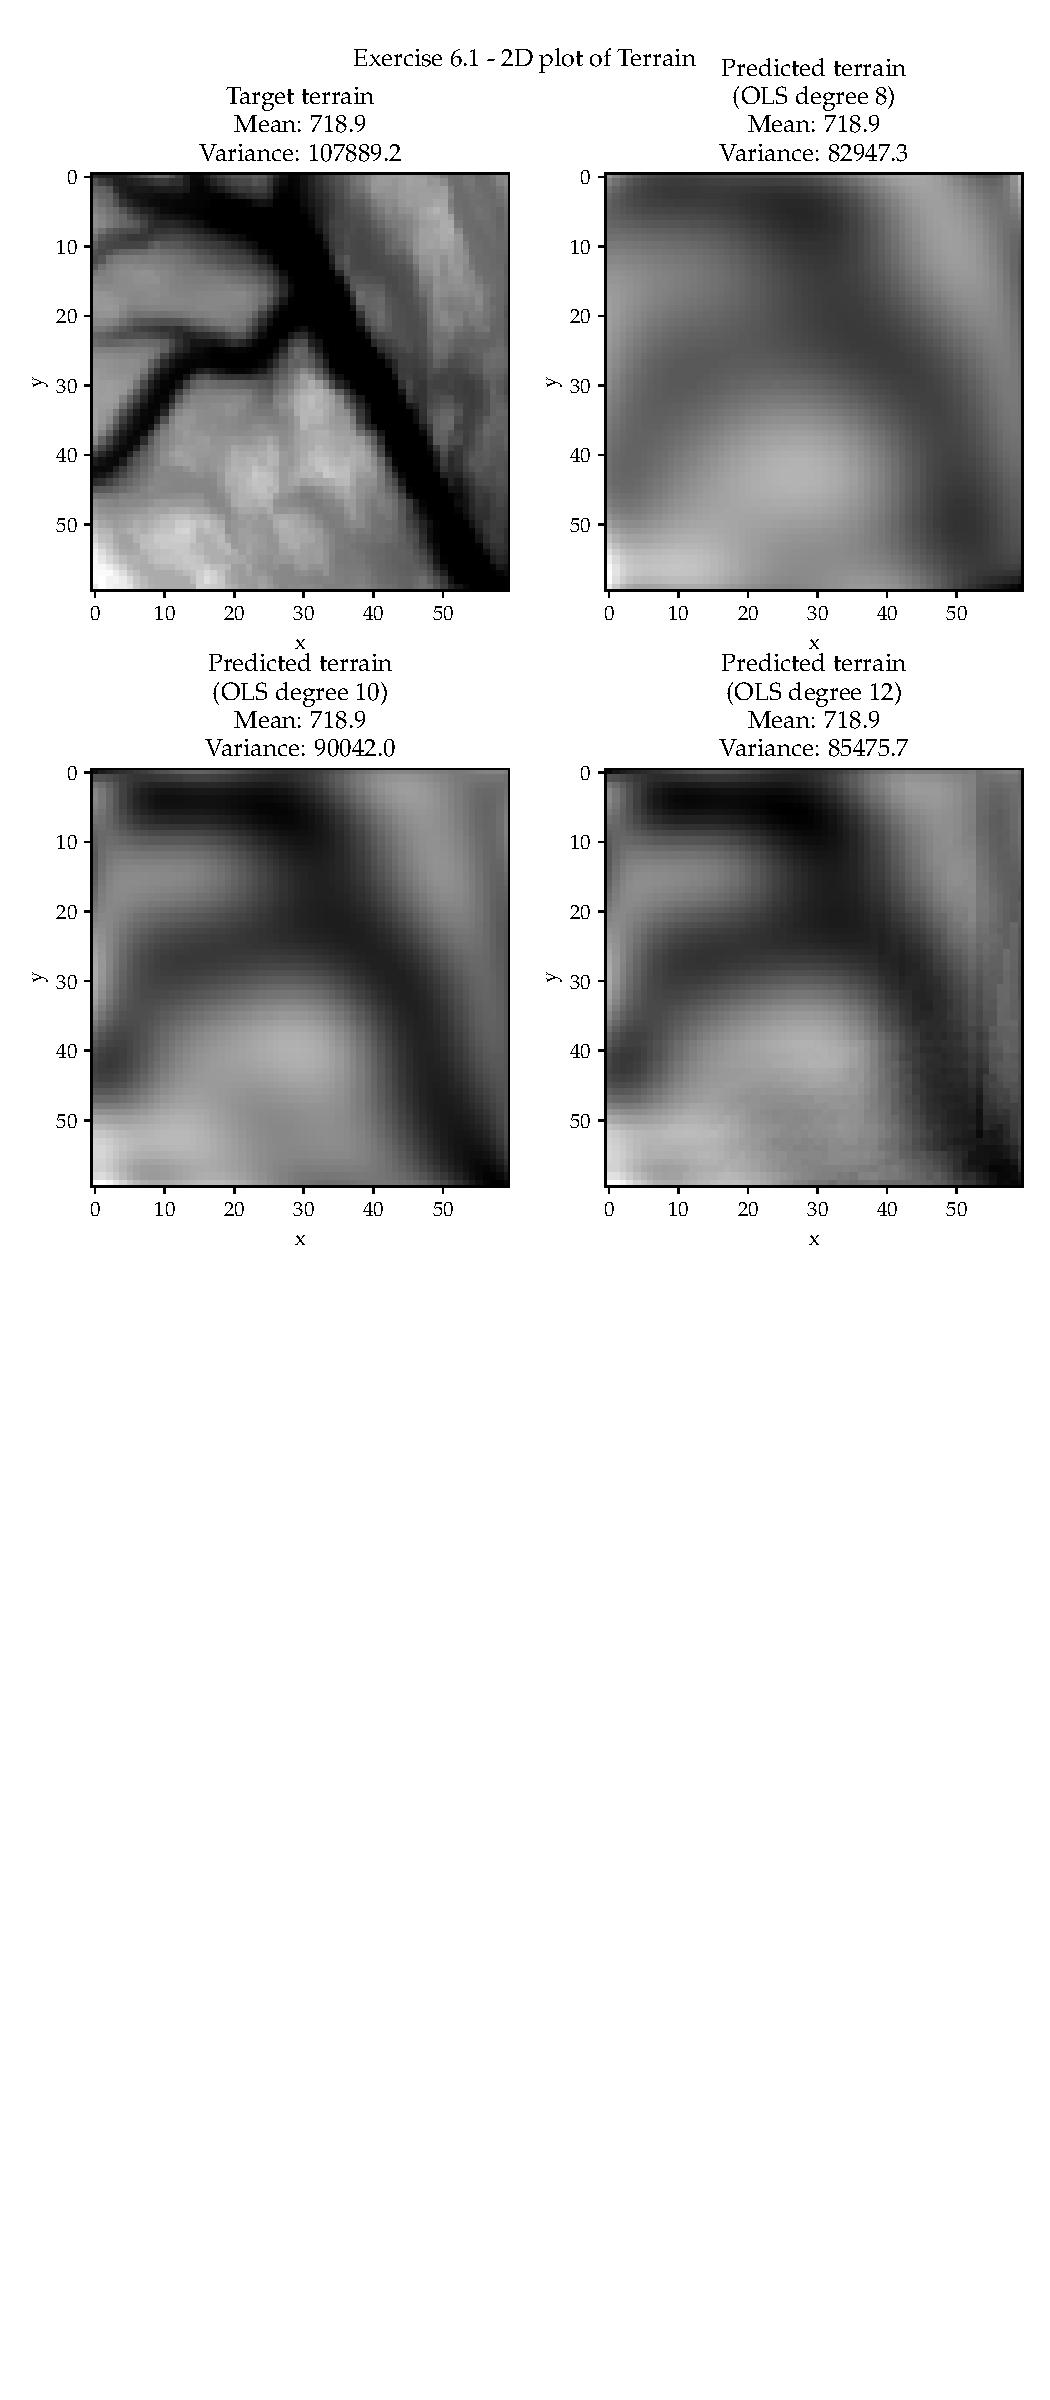
\includegraphics[scale=0.95]{figures/EX6_EX1_target_terrain_and_OLS_prediction_2D.pdf}
  \label{fig:EX6_1_OLS_2D}
\end{figure}

\begin{figure}
  \centering
  \caption{3D plot showing the produced product from models at degree9-12}
  \hspace*{-1.2cm}  
  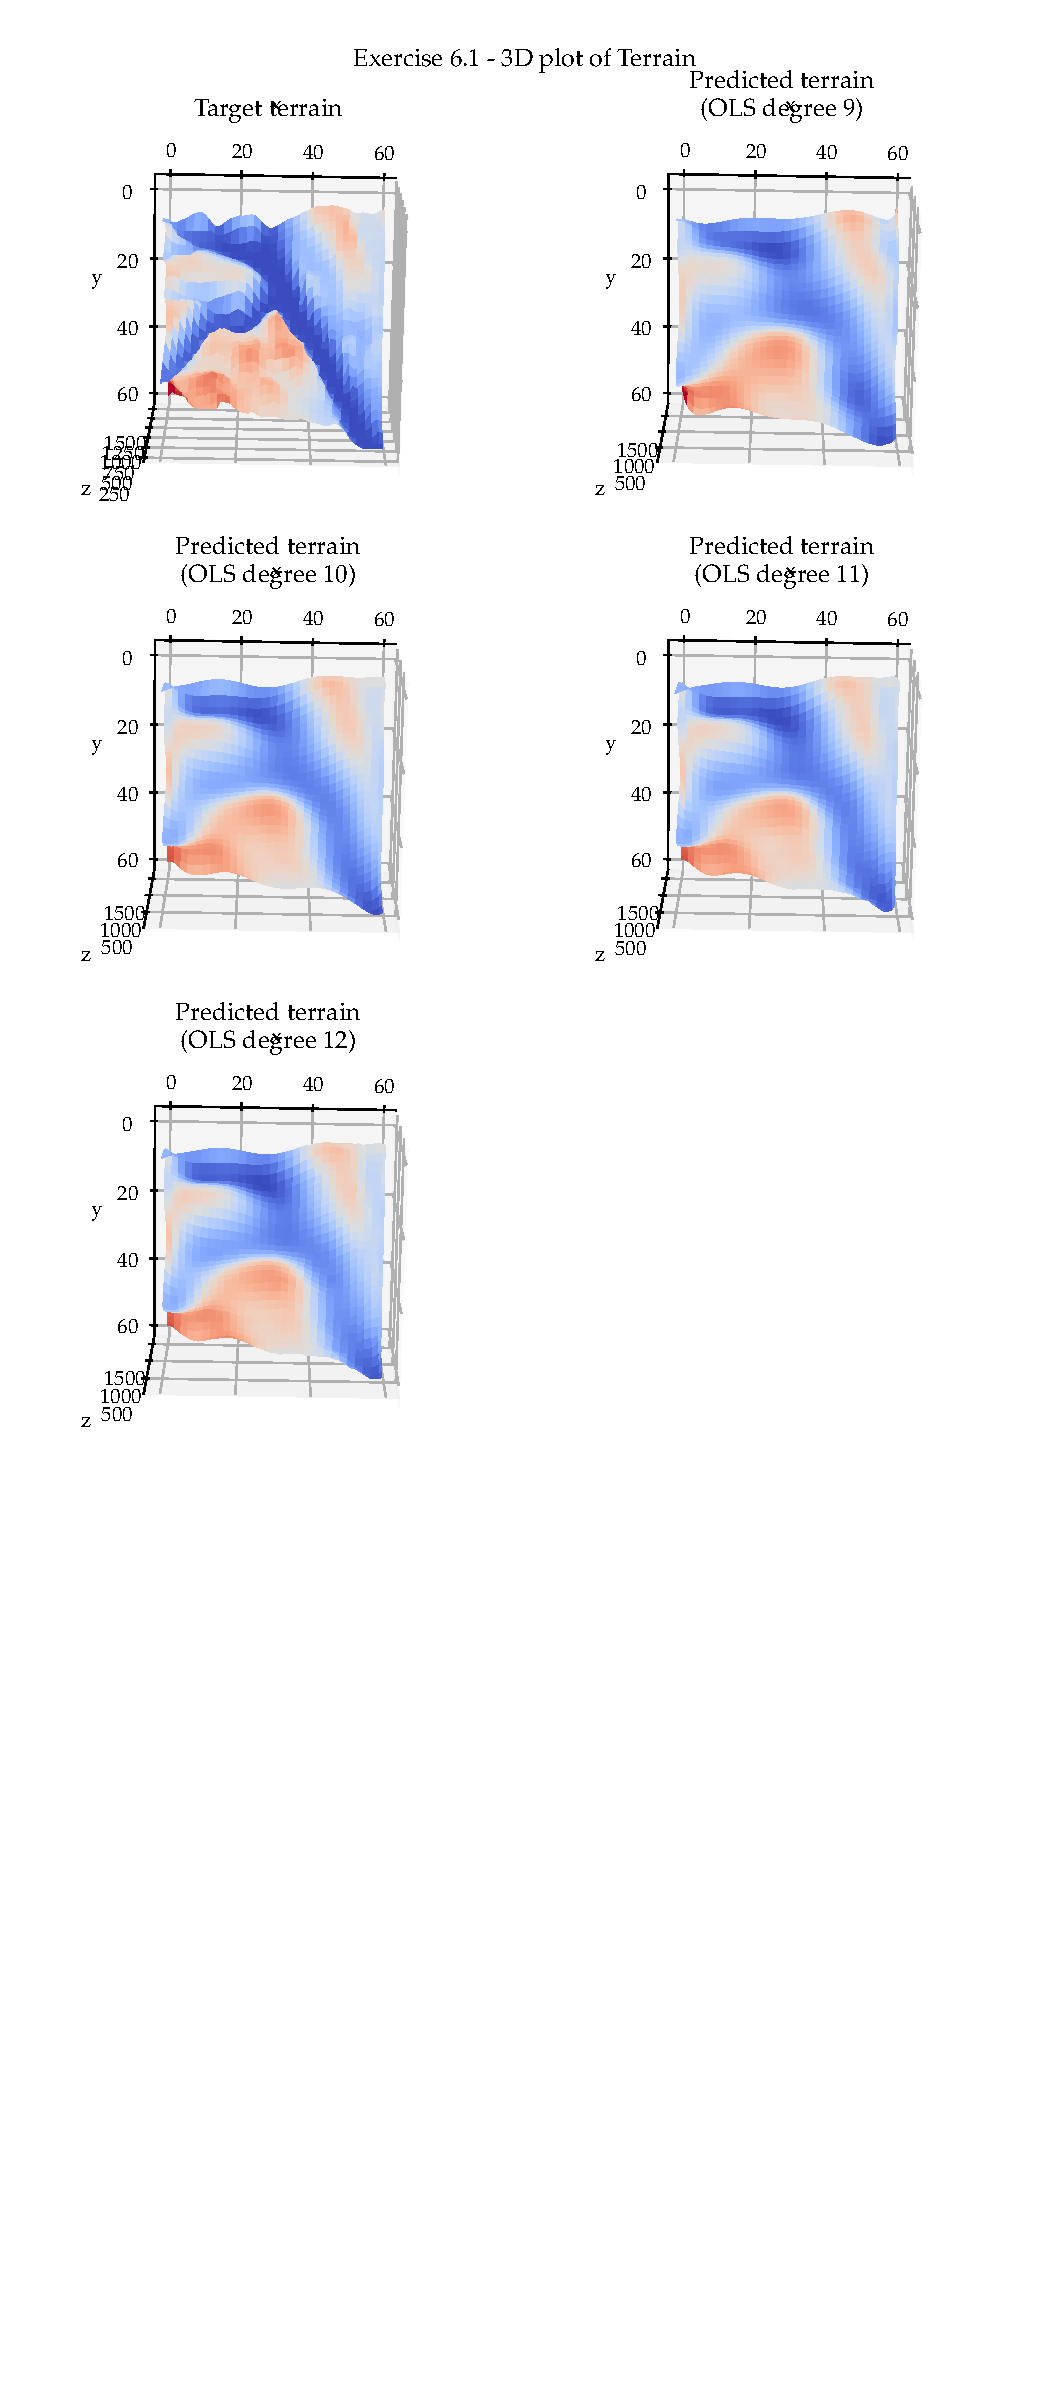
\includegraphics[scale=0.95]{figures/EX6_EX1_target_terrain_and_OLS_prediction_3D.pdf}
  \label{fig:EX6_1_OLS_3D}
\end{figure}


\section*{Appendix\label{sec:A}}
\textbf{TODO} her skal det ligge link til et github repo.

\newpage
\newpage

\bibliographystyle{plain}
\bibliography{bibliography}




\end{document}


% Local Variables:
% TeX-engine: xetex
% End:
